\documentclass[a4paper,fleqn]{cas-sc}

\usepackage[utf8]{inputenc}
\usepackage[T5,T1]{fontenc}
% ── Native Vietnamese Typography Support for Legal Vernacular Names ─
\DeclareTextFontCommand{\textvn}{\fontencoding{T5}\selectfont}

\usepackage[numbers,sort&compress]{natbib}
\usepackage{amsmath,amssymb,amsfonts,amsthm}
\usepackage{graphicx}
\usepackage{booktabs}
\usepackage{tabularx}
\usepackage{float}
\usepackage[section]{placeins}
\usepackage{hyperref}
\usepackage{tikz}
\usepackage{url}
\usepackage{multirow}
\usepackage{array}
\usepackage{microtype}
\microtypesetup{expansion=false}
\usepackage{makecell}
\usepackage{algorithm}
\usepackage{algpseudocode}
\usepackage{subcaption}

% ── Hyperref Academic Configuration ─────────────────────────────────
\hypersetup{
    colorlinks=true,
    linkcolor=cyan!80!black,
    citecolor=cyan!80!black,
    urlcolor=cyan!80!black
}

\newcommand{\orcidicon}[1]{\href{https://orcid.org/#1}{\texorpdfstring{%

\begin{tikzpicture}[baseline=-0.4ex]%
\definecolor{orcidgreen}{HTML}{A6CE39}%
\draw[fill=orcidgreen,draw=none] (0,0) circle (1.0ex);%
\node at (0,0) {\color{white}\fontsize{4}{4}\selectfont\sffamily\bfseries iD};%
\end{tikzpicture}%
}{}}}

% ── Footer Suppression for Elsevier CAS Template ───────────────────
\ExplSyntaxOn
\cs_set:Npn \__first_footerline: {}
\cs_set:Npn \__first_foot: {}
\cs_set:Npn \__cas_foot: {}
\ExplSyntaxOff

\let\printorcid\relax

% ── Strict Taxonomic & Author Hyphenation Prevention ─────────────────
\hyphenation{Afzelia Guibourtia Pterocarpus Dalbergia Sindora}

\newtheorem{definition}{Definition}
\newtheorem{proposition}{Proposition}
\newtheorem{lemma}{Lemma}
\newtheorem{observation}{Observation}

\begin{document}

\let\WriteBookmarks\relax
\def\floatpagepagefraction{1}
\def\textpagefraction{.001}

% Short title & Short authors for running headers
\shorttitle{Mitigating Specimen-Level Data Leakage in Wood Species Identification}
\shortauthors{\mbox{V.-A. Le} et al.}

% Main title
\title [mode = title]{Mitigating Specimen-Level Data Leakage in Wood Species Identification: A Multi-Paradigm Partitioning Benchmark and Combinatorial Governance Framework}

% Authors & Affiliations
\author[1]{\mbox{Viet-Anh Le}\orcidicon{0009-0003-5748-0439}}

\author[1]{Khanh Nguyen-Trong\orcidicon{0000-0001-5175-8805}}
\cormark[1]

\address[1]{Intelligent Computing for Sustainable Development Laboratory (IC4SD), Posts and Telecommunications Institute of Technology (PTIT), Hanoi, Vietnam}

\cortext[1]{ Corresponding author.\\ \hspace*{2.2em}\textit{E-mail addresses:} \href{mailto:khanhnt@ptit.edu.vn}{khanhnt@ptit.edu.vn} (K. Nguyen-Trong), \href{mailto:anhlv.b23kh002@stu.ptit.edu.vn}{anhlv.b23kh002@stu.ptit.edu.vn} (\mbox{V.-A.} Le)}

\begin{abstract}
In computer-vision-based biological specimen identification, data leakage across physical specimen boundaries -- termed \mbox{Same-Specimen-Picture Bias} (SSPB) or Class~IV Boundary Leakage -- causes deep learning models to exploit non-taxonomic surface preparation artifacts (saw striations, sanding abrasions, vignetting) rather than authentic diagnostic morphology. Under conventional random image-level partitioning, this shortcut learning produces inflated near-perfect test accuracy that degrades substantially upon deployment to novel physical specimens. Although standard group-aware partitioning isolates physical specimens, it treats all taxa homogeneously, frequently triggering severe minority-class performance collapse under deep neural fine-tuning.

To address this challenge from a data-centric governance perspective, we formalize the Specimen-Centric Data Protocol (SCDP) targeting two core governance objectives: physical subfolder integrity (as an asymptotic theoretical target, $\mathrm{SLR} \to 0\%$) and 100\% Class Coverage Rate ($\mathrm{CCR}$), evaluated through an operational Specimen Leakage Risk ($\mathrm{SLR}$) metric. We formalize the discrete integer condition for whole-block partitioning: strict 3-way specimen disjointness with full class coverage is mathematically impossible unless every taxon possesses at least three physical blocks ($|\mathcal{G}_c| \ge 3$). In real-world small-sample datasets ($|\mathcal{G}_c| < 10$), volume balance constraints and out-of-distribution (OOD) feature separation induce operational boundary friction, forcing standard solvers to trigger image fallbacks on boundary blocks to avoid class starvation. By employing a zero-training 1-nearest-neighbor benchmark on frozen deep representations, we isolate the causal impact of dataset partitioning from neural-network training stochasticity. We systematically benchmark 13 partitioning protocols across six algorithmic paradigms on an 18-species macroscopic wood dataset (curated from an archival repository of 20,470 images across 210 blocks into a standardized benchmark of 6,410 images across 116 quality-verified canonical blocks) using a ``Three Pillars'' evaluation framework comprising 16 quantitative metrics. Furthermore, to accommodate taxon-specific morphological heterogeneity, we introduce a Multi-Objective Simulated Annealing Meta-Selector (CEGS-Split: \textbf{C}ombinatorial \textbf{E}ntity \textbf{G}overnance \textbf{S}trategy for Dataset \textbf{Split}ting) that optimizes class-wise solver assignments over an $11^{18}$ search space.

Empirical evaluations across five random seeds reveal that naive random splitting inflates top-1 accuracy by $+2.13$ percentage points (pp) and macro-F1 by $+4.52$~pp relative to the standard group-disjoint baseline (\textsf{Stratified Group Split}), with the performance gap expanding to $+9.10$~pp in accuracy and $+16.75$~pp in Macro-F1 relative to global feature-disjoint separation (\textsf{DataSAIL Specimen-Level ILP}, Welch's $t$-test $p = 2.28 \times 10^{-6}$). However, unconstrained global ILP inherently causes minority-class starvation, collapsing hardest-class performance ($\mathrm{F1}_{\text{Hardest}} = 0.1193$) and class coverage ($\mathrm{CCR} = 88.9\%$). In contrast, the proposed Meta-Selector achieves an optimal Pareto compromise: it compresses empirical boundary leakage from $100\%$ down to the empirical baseline floor ($\mathrm{SLR} = 6.0\%$, where only 7 boundary blocks across 116 canonical blocks undergo image-level fallback to guarantee 3-way split representation) while strictly guaranteeing $\mathrm{CCR} = 100.0\%$ and preventing hardest-class collapse ($\mathrm{F1}_{\text{Hardest}} = 0.7407$ on frozen features, and providing a robust floor safeguard of $\ge 34.2\%$ under end-to-end neural fine-tuning across four distinct architectures). Formulation ablation confirms that continuous penalty terms fail to suppress leakage, whereas combinatorial meta-selection establishes rigorous Pareto-optimal governance. The governed benchmark dataset, cryptographic SHA-256 partition manifests, and reproducible evaluation suite are openly released.
\end{abstract}

\begin{keywords}
Data leakage \sep \mbox{Same-Specimen-Picture Bias} \sep Wood species identification \sep DataSAIL \sep Multi-objective optimization \sep Simulated annealing \sep Out-of-distribution benchmark \sep Data governance
\end{keywords}

\maketitle

%======================================================================
\section{Introduction}
\label{sec:intro}
%======================================================================

Automated visual identification powered by deep representations has emerged as an essential tool across botanical classification, medical imaging, agricultural diagnostics, and forensic material inspection~\cite{woodreview,rosadasilva2022,varoquaux2022,roberts2021}. In forestry science and international timber trade regulation, rapid macroscopic wood species identification is critical for enforcing the Convention on International Trade in Endangered Species of Wild Fauna and Flora (CITES Appendix~II)~\cite{cites}, verifying legal supply chains, and combating illegal deforestation~\cite{dormontt2015,song2025,liu2025}. Computer vision promises field-deployable, non-destructive screening that supplements labor-intensive xylotomy at customs checkpoints. Yet, despite reported laboratory classification accuracies exceeding 95--99\% in recent literature~\cite{song2025,fabijanska2021,wu2021}, such systems frequently suffer severe performance degradation once evaluated on novel physical specimens~\cite{ravindran2019,ravindran2020,ravindran2021,ravindran2022}.

We argue that a primary driver of this systemic deployment failure is the absence of rigorous data-governance standards during dataset construction and partitioning in applied computer vision. We formalize this challenge under a unified framework: \textbf{Physical Entity-Centric Visual Classification (PECVC)}. PECVC encompasses any visual recognition problem in which individual physical entities -- timber blocks, patient tissue specimens, agricultural plants, or alloy samples -- yield multiple correlated image captures. In prevailing PECVC workflows, researchers photograph physical specimens, crop high-resolution fields of view into image patches, and store them in flat directory structures organized solely by target species~\cite{east2025}. The resulting pool is subsequently partitioned via conventional \emph{random image-level splits}. This procedure discards physical object provenance: sub-images originating from the same physical entity are distributed across training, validation, and test sets.

This partitioning flaw induces \textbf{\mbox{Same-Specimen-Picture Bias} (SSPB)}~\cite{figueroamata2022}, more broadly identified as \textbf{specimen-level data leakage}~\cite{varoquaux2022,roberts2021,kapoor2023}. Crucially, as surveyed by Kapoor and Narayanan~\cite{kapoor2023} across 329 empirical machine-learning studies spanning 17 scientific fields and conceptualized by Varoquaux and Cheplygina~\cite{varoquaux2022}, this vulnerability constitutes an acute manifestation of \emph{Class~IV Boundary Leakage}: a structural partitioning failure where train/test splits violate physical entity boundaries, remaining completely invisible under standard cross-validation while driving substantial performance overestimation. This failure mode is conceptually and mathematically isomorphic to cross-sectional unit leakage in panel econometrics~\cite{cerqua2026,babii2024} and spatial autocorrelation in geoscience~\cite{roberts2017}. Under random image-level partitioning, deep neural networks behave as opportunistic ``shortcut learners''~\cite{geirhos2020}: rather than learning species-discriminative anatomical traits (vessel-pore patterns, axial parenchyma arrangements, ray density), they exploit non-taxonomic surface artifacts, illumination gradients, and sensor fingerprints unique to individual physical specimens. High reported test accuracy then measures the model's ability to re-identify previously seen physical sources rather than recognize novel biological material.

\subsection{Mechanisms of Specimen-Level Data Leakage}
In macroscopic wood imagery, specimen leakage operates through three distinct physical mechanisms:
\begin{enumerate}
\item \textbf{Mechanism 1 (Geometric and Anatomical Continuity)}: Sub-images extracted from the same physical wood block share continuous anatomical trajectories -- matching growth-ring curvature, identical vessel-pore cluster geometry, and continuous parenchyma banding. Deep representations encode these spatial configurations as high-dimensional visual signatures of the individual specimen rather than the botanical species.
\item \textbf{Mechanism 2 (Acquisition and Illumination Fingerprints)}: Images captured within the same imaging session inherit identical sensor noise (photo-response non-uniformity), flash reflections, lens vignetting, color balance casts, and static shadows, allowing models to exploit acquisition parameters rather than biological morphology.
\item \textbf{Mechanism 3 (Surface Preparation Artifacts)}: Mechanical processing (sawing, planing, sanding) leaves specimen-unique micro-scratch densities, weathering cracks, and varnish absorption patterns, which serve as salient non-taxonomic shortcuts~\cite{geirhos2020}.
\end{enumerate}

\subsection{Taxon Heterogeneity and Combinatorial Partitioning}
Standard group-aware partitioning (e.g., \texttt{GroupKFold}, \texttt{StratifiedGroupKFold}) enforces physical specimen isolation but assumes all classes behave homogeneously. In biological datasets, taxa exhibit pronounced morphological divergence:
\begin{itemize}
\item \textbf{Uniform taxa} with homogeneous growth rings and consistent coloration (e.g., \textit{Guibourtia coleosperma}) are cleanly separated by linear centroid-distance metrics (Mahalanobis distance, Ward linkage).
\item \textbf{Outlier-prone taxa} with irregular heartwood/sapwood boundaries or severe weathering (e.g., \textit{Afzelia bella}) distort standard distance metrics and require adversarial density validation~\cite{adversarialvalidation} or integer programming to isolate anomalous specimens.
\item \textbf{Visually similar sibling species} within the same genus (e.g., \textit{Dalbergia oliveri} vs.\ \textit{Dalbergia cochinchinensis}) require graph-based isolation of near-duplicate feature neighborhoods to sever indirect similarity leakage.
\end{itemize}

Imposing a single global splitting algorithm across all 18 species inevitably forces suboptimal partitions for taxa whose empirical distributions violate that algorithm's assumptions. If each taxon $c \in \{1,\dots,C\}$ ($C=18$) selects its own splitting solver $m_c \in \{1,\dots,K\}$ from a candidate pool of $K=11$ solvers, the configuration space spans:
\begin{equation}
\mathcal{M} = K^{C} = 11^{18} \approx 5.5599 \times 10^{18}\ \text{candidate global partitions.}
\label{eq:comb_space}
\end{equation}
Exhaustive evaluation of Eq.~\eqref{eq:comb_space} is computationally intractable. Furthermore, global objectives such as Maximum Mean Discrepancy ($\mathrm{MMD}$) and hardest-class F1 must be evaluated on the assembled global dataset $\mathcal{D}(\boldsymbol{m}) = \bigcup_{c=1}^{C} \mathcal{D}_c(m_c)$, which motivates a combinatorial meta-heuristic search rather than independent per-class greedy selection.

Despite growing awareness of specimen-level leakage, prior studies exhibit three critical gaps: (i) the absence of a standardized, verifiable data-governance protocol with quantitative leakage risk metrics; (ii) the lack of controlled, multi-paradigm benchmarking that isolates dataset partition boundaries from model training stochasticity; and (iii) the inability of single global splitting solvers to accommodate taxon-specific morphological heterogeneity across diverse biological classes. This paper directly addresses these three limitations.

\subsection{Primary Contributions}
The main contributions of this work are fourfold:
\begin{itemize}
\item \textbf{Governed S3 Wood Benchmark Dataset}: An 18-species macroscopic tropical timber benchmark curated from an archival collection of 20,470 raw images across 210 physical specimen blocks into a standardized, balanced collection of 6,410 quality-controlled images across 116 verified canonical blocks spanning 5 botanical genera (including 8 CITES Appendix~II taxa), organized into immutable specimen subfolders with cryptographic SHA-256 partition manifests.
\item \textbf{Multi-Paradigm Benchmark under the Three Pillars Framework}: A systematic evaluation of 13 partitioning protocols across six algorithmic paradigms using 16 quantitative metrics spanning leakage minimization, out-of-distribution difficulty, and decision-boundary preservation, validated through a zero-training 1-NN representation-level benchmark and 80 end-to-end deep neural fine-tuning runs.
\item \textbf{Combinatorial Meta-Selector (CEGS-Split)}: A multi-objective Simulated Annealing framework optimizing class-wise solver assignments over an $11^{18}$ search space. CEGS-Split reconciles taxon-specific morphological divergence, compressing empirical boundary leakage to the empirical baseline floor ($\mathrm{SLR} = 6.0\%$, leaving only 7 boundary blocks split across 116 canonical blocks) while strictly guaranteeing 100\% Class Coverage Rate ($\mathrm{CCR}$) and acting as an indispensable floor safeguard against hardest-class collapse across multiple deep neural architectures.
\item \textbf{Combinatorial Boundary Analysis and SCDP Data Governance}: Formalization of the Specimen-Centric Data Protocol (SCDP) targeting physical specimen integrity alongside the Specimen Leakage Risk ($\mathrm{SLR}$) metric. We mathematically establish the necessary integer block condition for strict 3-way disjointness ($|\mathcal{G}_c| \ge 3$) and analytically characterize the operational boundary friction arising from discrete block allocation, volume ratios, and out-of-distribution separation in small-sample regimes ($|\mathcal{G}_c| < 10$).
\end{itemize}

The remainder of this paper is structured as follows. Section~\ref{sec:related} reviews related work. Section~\ref{sec:governance} formalizes the data governance protocol and the combinatorial meta-selector. Section~\ref{sec:setup} details the experimental setup and representation-level evaluation. Section~\ref{sec:results} presents the empirical results, ablation, and diagnostic analysis. Section~\ref{sec:discussion} outlines practical guidelines and limitations. Section~\ref{sec:conclusion} concludes the paper.

%======================================================================
\section{Related Work}
\label{sec:related}
%======================================================================

\subsection{Specimen Leakage and \mbox{Same-Specimen-Picture Bias}}
Data leakage is recognized as a major cause of reproducibility failures in computational science~\cite{kaufman2012,kapoor2023}. Kapoor and Narayanan~\cite{kapoor2023} reviewed over 600 machine-learning-based scientific papers across 30 disciplines, finding that leakage-driven overoptimism systematically distorts reported performance. In plant vision, Figueroa-Mata et al.~\cite{figueroamata2022} conceptualized \mbox{Same-Specimen-Picture Bias} (SSPB), warning that evaluating models on sub-images of wood blocks present in the training set produces heavily biased accuracy. Rosa da Silva et al.~\cite{rosadasilva2022} corroborated that multi-view wood datasets routinely ignore physical sample boundaries. In timber forensics, Ravindran et al.~\cite{ravindran2019,ravindran2021,ravindran2022} and Wiedenhoeft~\cite{wiedenhoeft2011} documented deployment gaps of 10\% to 25\% between xylarium benchmarks and field tests. However, prior field evaluations conflated specimen leakage with external illumination shifts and sensor changes; our framework isolates pure specimen-level leakage under controlled feature representations.

\subsection{Cross-Disciplinary Parallels: Econometrics and Spatial Statistics}
Boundary leakage is structurally isomorphic across multiple quantitative disciplines. In financial econometrics, L{\'o}pez de Prado~\cite{lopezdeprado2018} formalized Purged Cross-Validation (PCV) to eliminate temporal overlap between train and test splits. In panel data econometrics, Cerqua et al.~\cite{cerqua2026} audited 480 machine learning models across 3,058 U.S. counties, demonstrating that random partitioning inflates predictive accuracy by over 17\% in MSE and 0.05 in AUC by conflating cross-sectional unit leakage (observing the same county in both splits) with temporal leakage. Babii et al.~\cite{babii2024} established that preserving panel dependency structures requires structured block sampling. In spatial statistics, Roberts et al.~\cite{roberts2017} showed that spatial autocorrelation inflates predictive skill unless spatial blocking is applied. Table~\ref{tab:cross_domain_inflation} summarizes reported performance inflation margins across diverse fields, confirming that specimen leakage in biological computer vision mirrors broader empirical phenomena. These cross-domain findings motivate our controlled isolation of the specimen boundary leakage effect in biological vision.

\begin{table}[pos=htbp]
\centering
\footnotesize
\setlength{\tabcolsep}{4pt}
\renewcommand{\arraystretch}{1.15}
\caption{Cross-domain empirical performance inflation induced by entity-level boundary leakage across scientific fields.}
\label{tab:cross_domain_inflation}
\resizebox{\textwidth}{!}{%
\begin{tabular}{llll}
\toprule
\makecell[l]{\textbf{Scientific}\\\textbf{Domain}} & \makecell[l]{\textbf{Physical Entity}\\\textbf{Unit}} & \makecell[l]{\textbf{Benchmark}\\\textbf{Reference}} & \makecell[l]{\textbf{Observed Inflation}\\\textbf{Margin}} \\
\midrule
Retinal Ophthalmology & Patient / Eye Volume & Tampu et al.~\cite{tampu2022} & $+5.0$ to $+30.0$ pp accuracy \\
Neuroimaging (Brain MRI) & Subject / Scan Volume & Yagis et al.~\cite{yagis2021} & Slide acc.\ up to $+29.0$ pp; $+25.4$ pp Macro-F1 \\
COVID-19 Radiography & Patient / Hospital Site & Roberts et al.~\cite{roberts2021} & $+12.0$ to $+24.0$ pp diagnostic accuracy \\
Macro Panel Econometrics & County / Geographic Unit & Cerqua et al.~\cite{cerqua2026} & $+17.2\%$ MSE underest.; $+0.05$ AUC \\
\midrule
\textbf{Macroscopic Wood ID (Ours)} & \textbf{Timber Specimen Block} & \textbf{This Study (Table~\ref{tab:master_results})} & \textbf{+9.10 pp Acc; +16.75 pp F1} \\
\bottomrule
\end{tabular}%
}
\end{table}

\subsection{Data Partitioning Paradigms and DataSAIL}
Standard machine-learning libraries provide group-aware utilities like \texttt{GroupKFold} and \texttt{StratifiedGroupKFold}~\cite{scikit}, which partition datasets based on discrete group tags (e.g., patient, batch, specimen). However, these conventional tools partition groups uniformly without considering continuous feature-space geometry or out-of-distribution metric shifts. To bridge this gap, Joeres et al.~\cite{joeres2025} introduced DataSAIL (Data Splitting Against Information Leakage), a seminal framework formulating dataset splitting as an integer linear program (ILP) that minimizes inter-split feature similarity:
\begin{equation}
\min_{\pi} \sum_{i \neq j} \mathbb{1}[\pi(i) \neq \pi(j)] \cdot S(i, j) \cdot w_i \cdot w_j,
\label{eq:datasail_objective}
\end{equation}
where $\pi(i)$ denotes partition assignment, $S(i,j)$ represents pairwise feature similarity, and $w_i, w_j$ denote sample importance weights. DataSAIL was primarily designed for chemoinformatics, drug-target interaction, and computational biology, where isolating highly similar molecular scaffolds is paramount. In its canonical formulation, DataSAIL optimizes a single global feature-similarity objective without explicitly imposing hard constraints on minority-class presence across all splits ($\mathrm{CCR} = 100\%$) or worst-case class recall ($\mathrm{F1}_{\text{Hardest}}$). When applied directly to multi-class biological identification tasks containing rare or endangered taxa (such as CITES wood identification), global unconstrained ILP naturally concentrates outlier specimens of minority taxa into evaluation splits to minimize cross-split similarity, inadvertently depriving the training split of representative samples. Our governance framework builds directly upon DataSAIL's core information-theoretic insight, integrating its leakage loss as a vital optimization anchor while establishing combinatorial class-wise meta-selection to rigorously safeguard minority-class survival.

%======================================================================
\section{Specimen-Centric Data Governance and Proposed Framework}
\label{sec:governance}
%======================================================================

\subsection{Notation and Specimen Leakage Risk (SLR)}
Let $\mathcal{D} = \{(x_i, y_i, g_i)\}_{i=1}^N$ denote a dataset of $N$ images, where $x_i \in \mathcal{X}$ is an RGB image, $y_i \in \{1, \dots, C\}$ is the botanical species label ($C=18$), and $g_i \in \mathcal{G}$ represents the physical specimen block identifier. A data partition $\pi: \mathcal{D} \to \{\text{Train}, \text{Val}, \text{Test}\}$ maps each sample to a partition split. We quantify physical specimen leakage via the \textbf{Specimen Leakage Risk (SLR)}:
\begin{equation}
\mathrm{SLR}(\pi) = \frac{\left|\{g \in \mathcal{G} \mid \exists\, x, x' \in g \text{ s.t. } \pi(x) \neq \pi(x')\}\right|}{|\mathcal{G}|} \times 100\%,
\label{eq:slr}
\end{equation}
where $\mathrm{SLR}=0.0\%$ denotes complete physical specimen isolation across all partition splits.

\begin{definition}[SCDP Data Governance Objectives]
An ideal dataset partition $\pi^*$ strictly satisfies the Specimen-Centric Data Protocol if and only if it complies with two verifiable governance conditions:
\begin{enumerate}
\item[(i)] \textbf{Subfolder Integrity (Zero Specimen Leakage)}: Every image originating from the same physical specimen $g \in \mathcal{G}$ belongs exclusively to an identical split:
\begin{equation}
\forall g \in \mathcal{G}, \quad \pi(x_i) = \pi(x_j) \quad \forall\, x_i, x_j \in g \iff \mathrm{SLR}(\pi^*) \equiv 0.0\%.
\label{eq:subfolder_integrity}
\end{equation}
\item[(ii)] \textbf{Class Coverage Rate (CCR)}: Every species $c \in \{1, \dots, C\}$ is represented across Train, Validation, and Test:
\begin{equation}
\mathrm{CCR}(\pi) = \frac{\left|\{c \in \{1,\dots,C\} \mid c \text{ present in Train, Val, and Test}\}\right|}{C} \times 100\% \equiv 100.0\%.
\label{eq:ccr}
\end{equation}
\end{enumerate}
\end{definition}

\begin{lemma}[Necessary Condition for Strict Block Disjointness with Full Class Coverage]
\label{lem:block_condition}
Let $\mathcal{D}$ be partitioned into $S \ge 2$ pairwise disjoint splits ($S=3$ for Train, Validation, and Test) such that $\pi: \mathcal{D} \to \{1,\dots,S\}$. A partition strictly satisfies Subfolder Integrity ($\mathrm{SLR}(\pi) \equiv 0.0\%$) and complete Class Coverage ($\mathrm{CCR}(\pi) \equiv 100.0\%$) only if every botanical taxon $c \in \{1,\dots,C\}$ possesses at least $S$ distinct physical specimen blocks:
\begin{equation}
\forall c \in \{1,\dots,C\}, \quad |\mathcal{G}_c| \ge S.
\end{equation}
\end{lemma}
\begin{proof}
By the definition of complete Class Coverage ($\mathrm{CCR} \equiv 100.0\%$), for every taxon $c$ and each split $s \in \{1,\dots,S\}$, there must exist at least one sample $x_s \in \mathcal{D}$ such that $y(x_s) = c$ and $\pi(x_s) = s$. Let $g(x) \in \mathcal{G}_c$ denote the physical specimen block containing sample $x$. Under strict Subfolder Integrity ($\mathrm{SLR} \equiv 0.0\%$), every specimen block maps exclusively to a single split, implying $g \cap \pi^{-1}(s) \neq \emptyset \implies g \subseteq \pi^{-1}(s)$. Because the splits are mutually disjoint ($\pi^{-1}(s) \cap \pi^{-1}(s') = \emptyset$ for $s \neq s'$), the physical specimen blocks $g(x_1), g(x_2), \dots, g(x_S)$ must be mutually distinct entities. Consequently, $|\mathcal{G}_c| \ge S$. For a 3-way partition (Train, Val, Test), this requires $|\mathcal{G}_c| \ge 3$ physical blocks per taxon.
\end{proof}

\begin{observation}[Integer-Partition Feasibility and Empirical Fallback Leakage]
\label{obs:trilemma}
While Lemma~\ref{lem:block_condition} establishes the theoretical existence condition ($|\mathcal{G}_c| \ge 3$), small-sample biological datasets ($|\mathcal{G}_c| < 10$) impose severe integer-knapsack friction when simultaneously satisfying:
\begin{enumerate}
\item[(a)] Target volume proportions across splits (e.g., $65\%/18\%/17\%$);
\item[(b)] Heterogeneous block capacities (specimen blocks yield unequal numbers of usable image patches);
\item[(c)] Out-of-distribution (OOD) distributional divergence or boundary preservation across splits.
\end{enumerate}
When physical blocks are indivisible discrete units, finding a 3-way partition that strictly satisfies all volume ratios while keeping every class represented across all three splits is frequently integer-infeasible. In standard group-partitioning implementations (e.g., \texttt{StratifiedGroupKFold}) and group-aware heuristics, this integer infeasibility is resolved through \textbf{boundary image-level fallbacks}: a minimal subset of boundary blocks are split across partitions to prevent empty splits and preserve $\mathrm{CCR} \equiv 100.0\%$. In our canonical benchmark of 116 physical blocks, exactly 7 boundary blocks are partitioned via fallback across splits, yielding an empirical baseline leakage floor of $\mathrm{SLR} = 7 / 116 \approx 6.0\%$. Conversely, enforcing $\mathrm{SLR} \equiv 0.0\%$ by disallowing boundary fallbacks (as seen in unconstrained DataSAIL Specimen ILP) forces the omission of minority taxa from evaluation splits, causing class coverage collapse ($\mathrm{CCR} = 88.9\%$) and worst-case boundary failure ($\mathrm{F1}_{\text{Hardest}} = 0.1193$). Practical data governance in small-sample regimes therefore operates as a Pareto optimization: compressing empirical boundary leakage to its feasible baseline floor ($6.0\%$) while strictly guaranteeing $100\%$ class coverage.
\end{observation}

\subsection{Taxonomy of Partitioning Protocols and Candidate Solver Pool}
To accommodate morphological divergence across diverse taxa, candidate class-wise partitions are drawn from a comprehensive candidate pool of $K=11$ algorithmic solvers $\mathcal{K} = \{\text{PP1}, \dots, \text{PP11}\}$. We draw an essential methodological distinction between \textbf{standalone baseline evaluation} (Category II, where continuous solvers are tested on raw image vectors to quantify unconstrained metric leakage) versus \textbf{block-governed candidate instantiation within CEGS-Split} (Category IV, where continuous solvers are strictly projected onto specimen centroids to preserve physical block integrity):
\begin{itemize}
\item \textbf{Continuous Feature-Space Solvers}:
  \begin{itemize}
  \item \textbf{PP1: Fixed Mahalanobis Stratification}: Computes distance quantiles to a static class centroid $\boldsymbol{\mu}_c$. In standalone Category II evaluation on raw image patches, this unconstrained sorting disperses subfolders across splits ($\mathrm{SLR} = 100.0\%$). In CEGS-Split, it is block-governed by evaluating Mahalanobis distances over pooled specimen centroids $\bar{\boldsymbol{\phi}}_g$, assigning intact physical blocks;
  \item \textbf{PP2: Iterative Mahalanobis Allocation}: Dynamically re-estimates class covariance and centroid upon allocating each specimen block, preventing outlier masking in skewed distributions;
  \item \textbf{PP3: Density-Adaptive Mahalanobis Banding}: Weights Mahalanobis distances using local kernel density estimates across specimen centroids;
  \item \textbf{PP5: Cosine Feature Graph Partitioning}: Constructs a $k$-NN cosine similarity graph and computes min-cut graph partitions. In standalone Category II evaluation on raw images, it yields $\mathrm{SLR} = 90.3\%$; inside CEGS-Split, the graph is constructed strictly over specimen block centroids $\bar{\boldsymbol{\phi}}_g$.
  \end{itemize}
\item \textbf{Specimen-Group-Aware Discrete Solvers (Block-Disjoint by Design)}:
  \begin{itemize}
  \item \textbf{PP4: Hierarchical Agglomerative Partitioning}: Performs Ward's minimum variance clustering on specimen centroids to cut discrete subtree clusters;
  \item \textbf{PP6: Spectral Graph Bipartitioning}: Bipartitions specimen similarity graphs using the Fiedler vector of the normalized graph Laplacian;
  \item \textbf{PP7: Adversarial Density Validation}~\cite{adversarialvalidation}: Trains a binary domain discriminator over specimen representations to route distribution-divergent blocks to evaluation splits;
  \item \textbf{PP8: Stratified Group Allocation}: Extends \texttt{StratifiedGroupKFold} to optimize multi-objective block disjointness while balancing class sample sizes;
  \item \textbf{PP9: Agglomerative Stratified Banding}: Combines specimen clustering with geometric radial distance bands (Near, Mid, Far);
  \item \textbf{PP10: Support Vector Margin Partitioning}: Fits a one-class SVM hyperplane to specimen centroids, routing boundary-margin outliers to evaluation;
  \item \textbf{PP11: Specimen-Level Integer Linear Programming}: Solves the DataSAIL ILP objective over specimen centroids.
  \end{itemize}
\end{itemize}

We evaluate 13 partitioning protocols organized into four broad categories:
\begin{itemize}
\item \textbf{Category I: Naive Image-Level Baselines}: \textsf{Naive Random Image Split} and \textsf{Naive Stratified Image Split} sample individual images uniformly without group provenance ($\mathrm{SLR} \approx 100\%$). \textsf{DataSAIL Image-Level ILP} minimizes Eq.~\eqref{eq:datasail_objective} over individual images without enforcing specimen disjointness ($\mathrm{SLR} = 95.3\%$).
\item \textbf{Category II: Single Splitting Protocols}: Imposes a single algorithmic paradigm globally across all 18 taxa, spanning both continuous feature-space baselines (PP1, PP5) and group-aware baselines (Naive Specimen Group Split, PP8 Stratified Group Split, PP4 Hierarchical Ward, PP9 Stratified Banding, PP7 Adversarial Density Validation, and PP11 DataSAIL Specimen-Level ILP).
\item \textbf{Category III: Single-Objective Combinatorial Selector}: Selects per-class solvers independently to minimize DataSAIL loss in isolation, ignoring cross-taxa assembly balance.
\item \textbf{Category IV: Multi-Objective Combinatorial Meta-Selector (CEGS-Split, Proposed)}: Explores the $11^{18}$ space via Simulated Annealing to discover Pareto-optimal per-class assignments balancing leakage, OOD difficulty, and boundary preservation.
\end{itemize}

\subsection{The Three Pillars Evaluation Framework}
Table~\ref{tab:three_pillars} organizes 16 quantitative evaluation metrics into three complementary pillars to evaluate partitions comprehensively.

\begin{table}[pos=htbp]
\centering
\small
\setlength{\tabcolsep}{4pt}
\renewcommand{\arraystretch}{1.22}
\caption{The Three Pillars Evaluation Framework comprising 16 quantitative metrics categorized by governance role.}
\label{tab:three_pillars}
\begin{tabular}{cllp{8.2cm}}
\toprule
\textbf{\#} & \textbf{Metric Name} & \textbf{Role} & \textbf{Mathematical Definition / Evaluation Objective} \\
\midrule
\multicolumn{4}{l}{\textit{\textbf{Pillar 1: Information Leakage Minimization}}} \\
$M_1$ & DataSAIL Loss $L(\pi)$ & Anchor & $\displaystyle L(\pi) = \frac{1}{2} \sum_{\pi(x) \neq \pi(x')} \cos(\phi(x), \phi(x')) \cdot \kappa(x) \kappa(x')$ \\
$M_2$ & Inter-Split Similarity $\bar{S}_{\text{inter}}$ & Probe & $\displaystyle \bar{S}_{\text{inter}} = \frac{1}{|\mathcal{D}_{\text{Tr}}| |\mathcal{D}_{\text{Te}}|} \sum_{x \in \mathcal{D}_{\text{Tr}}, y \in \mathcal{D}_{\text{Te}}} \cos(\phi(x), \phi(y))$ \\
$M_3$ & Specimen Leakage Risk $\mathrm{SLR}$ & Probe & Fraction of physical blocks split across partitions (Eq.~\ref{eq:slr}) \\
$M_4$ & Pseudoreplication Index $\mathrm{PRI}$ & Probe & Proportion of co-specimen image pairs shared across Train/Test \\
\midrule
\multicolumn{4}{l}{\textit{\textbf{Pillar 2: Out-of-Distribution \& Partition Geometry}}} \\
$M_5$ & Max.\ Mean Discrepancy $\mathrm{MMD}$ & Anchor & $\displaystyle \mathrm{MMD}^2(\mathcal{D}_{\text{Tr}}, \mathcal{D}_{\text{Te}}) = \left\| \frac{1}{N_{\text{tr}}} \sum_{x} \phi(x) - \frac{1}{N_{\text{te}}} \sum_{y} \phi(y) \right\|_{\mathcal{H}}^2$ \\
$M_6$ & Silhouette Separation $S_{\text{split}}$ & Probe & Cosine silhouette coefficient across partition assignments $\in [-1, 1]$ \\
$M_7$ & Class Coverage Rate $\mathrm{CCR}$ & Constraint & Percentage of taxa present in Train, Val, and Test (Eq.~\ref{eq:ccr}) \\
$M_8$ & Split Volume Deviation $\Delta V$ & Probe & $\displaystyle \Delta V = \sum_{s \in \{\text{Tr}, \text{Val}, \text{Te}\}} \left| \frac{|\mathcal{D}_s|}{N} - r_s \right|$ relative to targets $(65/18/17\%)$ \\
\midrule
\multicolumn{4}{l}{\textit{\textbf{Pillar 3: Downstream Generalization \& Statistical Rigor}}} \\
$M_9$ & 1-NN Top-1 Accuracy & Probe & Classification accuracy of 1-NN on frozen unit embeddings $\phi(x)$ \\
$M_{10}$ & 1-NN Top-3 Accuracy & Probe & Proportion of test queries with ground-truth class in Top-3 neighbors \\
$M_{11}$ & Macro-Averaged F1 & Probe & Unweighted arithmetic mean of per-species F1-scores across 18 taxa \\
$M_{12}$ & Balanced Accuracy & Probe & Arithmetic mean of per-species sensitivity/recall across all 18 taxa \\
$M_{13}$ & Hardest Class F1 $\mathrm{F1}_{\text{Hardest}}$ & Anchor & Minimum per-species F1-score: $\min_{c \in \mathcal{C}} \mathrm{F1}_c$ (worst-case boundary) \\
$M_{14}$ & Wasserstein Divergence $W_1$ & Probe & Mean $L_1$ Earth Mover's Distance between split and global class priors \\
$M_{15}$ & Welch's $t$-test $p$-value & Probe & Two-sample unequal-variance test assessing significance vs.\ Naive \\
$M_{16}$ & Cohen's $d$ Effect Size & Probe & Standardized effect size quantifying leakage inflation vs.\ Naive \\
\bottomrule
\end{tabular}
\end{table}

\paragraph{Optimization Anchors vs.\ Independent Diagnostic Probes}
Within the Three Pillars Framework, the multi-objective fitness function in Eq.~\eqref{eq:multi_obj_fitness} selects exactly one foundational mathematical representative from each pillar as an active optimization anchor: $L_{\text{DataSAIL}}$ for Pillar~1 (information leakage suppression), $MMD$ for Pillar~2 (distributional separation), and $\mathrm{F1}_{\text{Hardest}}$ for Pillar~3 (worst-case boundary preservation). Restricting active meta-heuristic search to these three orthogonal anchors prevents optimization dilution, objective collinearity, and combinatorial instability. Crucially, the remaining 13 metrics (such as $PRI$, $\bar{S}_{\text{inter}}$, $S_{\text{split}}$, $W_1$, and Cohen's $d$) are strictly withheld from the optimization loop, serving as independent, non-participating diagnostic probes to evaluate and stress-test the discovered partitions post-hoc.

\subsection{Combinatorial Meta-Selector (CEGS-Split)}
Candidate global configurations $\boldsymbol{m} = (m_1, \dots, m_C)$ are evaluated on the assembled dataset $\mathcal{D}(\boldsymbol{m}) = \bigcup_{c=1}^{C} \mathcal{D}_c(m_c)$ via the multi-objective fitness function:
\begin{equation}
\mathrm{Fitness}(\boldsymbol{m}) = w_1 \cdot \left( \frac{L_{\text{DataSAIL}}(\boldsymbol{m})}{10^3} \right) - w_2 \cdot \left( 10 \cdot MMD(\boldsymbol{m}) \right) - w_3 \cdot \left( 10 \cdot \mathrm{F1}_{\text{Hardest}}(\boldsymbol{m}) \right),
\label{eq:multi_obj_fitness}
\end{equation}
with baseline weights $w_1=1.0, w_2=0.5, w_3=0.5$. The fitness function is formulated for minimization: positive terms penalize cross-split visual leakage ($L_{\text{DataSAIL}}$), while negative terms reward distributional separation ($MMD$) and hardest-class generalization ($\mathrm{F1}_{\text{Hardest}}$). Scaling constants ($10^{-3}$ for DataSAIL loss, $10$ for $MMD$ and $\mathrm{F1}_{\text{Hardest}}$) were established from empirical pilot evaluations to normalize each objective to approximately unit order of magnitude.

\paragraph{Leakage-Free Validation and Held-Out Test Integrity}
To eliminate any vulnerability to \emph{Meta-Leakage} or data snooping during optimization, the fitness function in Eq.~\eqref{eq:multi_obj_fitness} is strictly evaluated across the \textbf{Train-Validation interface} ($\mathcal{D}_{\text{Train}} \leftrightarrow \mathcal{D}_{\text{Val}}$). Specifically, $\mathrm{F1}_{\text{Hardest}}(\boldsymbol{m})$ and $MMD(\boldsymbol{m})$ measure performance on the validation split relative to training representations. The \textbf{Held-Out Blind Test split} $\mathcal{D}_{\text{Test}}$ remains completely unobserved, untouchable, and frozen throughout all $N_{\text{iter}} = 10{,}000$ annealing iterations, evaluated solely once upon convergence on the final locked partition $\boldsymbol{m}^*$. Furthermore, each taxon's candidate partition designates a deterministic \emph{swap target} (Validation or Test, documented in Appendix~\ref{app:taxon_mapping}), specifying which non-training partition receives outlier blocks to balance cross-split volume without human intervention. The optimization procedure is executed via Simulated Annealing as formalized in Algorithm~\ref{alg:cegs_split}. Candidate partitions for all taxa and solvers are pre-cached offline, enabling rapid evaluation during stochastic neighbor mutations.

\paragraph{Block-Governed Instantiation and Validation of Empirical SLR = 6.0\%}
A foundational operational principle of CEGS-Split is that all candidate solvers in pool $\mathcal{K}$ are implemented as \textbf{block-governed entity operators}. Even when a continuous metric (such as Fixed Mahalanobis PP1 or Iterative Mahalanobis PP2) or graph solver (Cosine Graph PP5) is selected for a given taxon, the algorithm does not operate on loose image pixels. Instead, all images belonging to each physical specimen block $g \in \mathcal{G}_c$ are first mean-pooled into a single block centroid representation:
\begin{equation}
\bar{\boldsymbol{\phi}}(g) = \frac{1}{|g|} \sum_{x \in g} \phi(x), \quad \forall g \in \mathcal{G}_c.
\end{equation}
The mathematical partitioning logic (whether distance quantile sorting in PP1/PP2, or min-cut bipartitioning in PP5) is subsequently executed over the discrete set of block centroids $\mathcal{G}_c$, allocating entire physical blocks to Train, Val, or Test. Consequently, when CEGS-Split assigns PP1 to \textit{Dalbergia oliveri} and \textit{Guibourtia coleosperma}, or PP2 to \textit{Dalbergia melanoxylon}, \textit{Pterocarpus erinaceus}, and \textit{Pterocarpus macrocarpus} (Table~\ref{tab:taxon_solver_mapping}), these solvers assign intact physical wood blocks rather than fragmenting subfolders.

This block-level pooling provides the exact mathematical justification for the empirical measurement of $\mathrm{SLR} = 6.0\%$: across the 116 canonical blocks, 109 blocks remain strictly whole-subfolder disjoint. The remaining 7 split blocks correspond precisely to the integer knapsack boundary fallbacks required to maintain 3-way split representation ($\mathrm{CCR} = 100.0\%$) across minority taxa with $|\mathcal{G}_c| \le 5$ (Observation~\ref{obs:trilemma}). Crucially, had PP1 and PP2 been executed at the raw unblocked image level, the 5 taxa adopting them (comprising 34 physical blocks out of 116) would have experienced complete subfolder dispersion, mathematically driving global leakage to $\mathrm{SLR} \ge 34 / 116 \approx 29.3\%$. The empirical global measurement of $\mathrm{SLR} = 6.0\%$ confirms that specimen-block integrity is rigorously preserved across all continuous and discrete solvers in the governed benchmark.

\begin{algorithm}[pos=htbp]
\caption{Combinatorial Simulated Annealing Meta-Selector (CEGS-Split)}
\label{alg:cegs_split}
\begin{algorithmic}[1]
\Require Dataset $\mathcal{D} = \{(x_i, y_i, g_i)\}_{i=1}^N$, taxa $\{1,\dots,C\}$, solver pool $\mathcal{K}=\{1,\dots,K\}$, weights $(w_1, w_2, w_3)$, initial temperature $T_0$, cooling rate $\alpha$, maximum iterations $N_{\text{iter}}$.
\Ensure Pareto-favorable partition configuration $\boldsymbol{m}^*$ and assembled dataset $\mathcal{D}(\boldsymbol{m}^*)$.
\State \textbf{Offline Pre-computation:} Compute and cache candidate splits $\mathcal{D}_c(k)$ for all $c \in \{1,\dots,C\}$ and $k \in \mathcal{K}$.
\State \textbf{Initialization:} Sample $\boldsymbol{m}^{(0)} \sim \mathcal{K}^C$; assemble candidate Train/Val splits $\mathcal{D}_{\text{Train}}(\boldsymbol{m}^{(0)}), \mathcal{D}_{\text{Val}}(\boldsymbol{m}^{(0)})$; compute $F^{(0)} \gets \mathrm{Fitness}(\boldsymbol{m}^{(0)})$ strictly on Validation; set $\boldsymbol{m}^* \gets \boldsymbol{m}^{(0)}, F^* \gets F^{(0)}, T \gets T_0$.
\For{$t = 1$ \textbf{to} $N_{\text{iter}}$}
    \State Select random taxon $c \sim \{1, \dots, C\}$ and alternative solver $k' \sim \mathcal{K} \setminus \{m_c^{(t)}\}$.
    \State Form candidate configuration $\boldsymbol{m}_{\text{cand}} \gets (m_1^{(t)}, \dots, m_c^{(t)} \gets k', \dots, m_C^{(t)})$.
    \State Assemble $\mathcal{D}(\boldsymbol{m}_{\text{cand}})$ from cache and evaluate $\Delta F \gets \mathrm{Fitness}(\boldsymbol{m}_{\text{cand}}) - F^{(t)}$ on Validation.
    \If{$\Delta F < 0$ \textbf{or} $\mathrm{rand}(0,1) < \exp\left(-\Delta F / \max(10^{-5}, T)\right)$}
        \State $\boldsymbol{m}^{(t+1)} \gets \boldsymbol{m}_{\text{cand}}$, $F^{(t+1)} \gets \mathrm{Fitness}(\boldsymbol{m}_{\text{cand}})$.
        \If{$F^{(t+1)} < F^*$}
            \State $\boldsymbol{m}^* \gets \boldsymbol{m}^{(t+1)}$, $F^* \gets F^{(t+1)}$.
        \EndIf
    \Else
        \State $\boldsymbol{m}^{(t+1)} \gets \boldsymbol{m}^{(t)}$, $F^{(t+1)} \gets F^{(t)}$.
    \EndIf
    \State $T \gets T \times \alpha$.
\EndFor
\State Evaluate locked held-out test split $\mathcal{D}_{\text{Test}}(\boldsymbol{m}^*)$ once for final reporting.
\State \Return $\boldsymbol{m}^*$ and assembled dataset $\mathcal{D}(\boldsymbol{m}^*)$.
\end{algorithmic}
\end{algorithm}

\paragraph{Computational Complexity and Annealing Schedule}
With candidate splits pre-cached offline for all taxa and candidate solvers, each stochastic mutation step requires $O(N)$ operations to reassemble the global candidate partition $\mathcal{D}(\boldsymbol{m}_{\text{cand}})$ from cache and $O(N \log N)$ for representation-level fitness evaluation (dominated by nearest-neighbor distance computation). The simulated annealing schedule adopts geometric temperature decay $T \gets T \times \alpha$ with initial temperature $T_0 = 1.0$, minimum temperature threshold $T_{\min} = 10^{-5}$, and decay parameter $\alpha = 0.9995$ over $N_{\text{iter}} = 10{,}000$ iterations.

%======================================================================
\section{Experimental Setup}
\label{sec:setup}
%======================================================================

\subsection{Dataset Curation, Optical Acquisition, and Governance Verification}
\paragraph{Two-Tier Data Architecture and Curation Pipeline}
To ensure methodological transparency and avoid data-distribution confounding, this study distinguishes between two distinct data tiers:
\begin{enumerate}
\item \textbf{Tier 1: Archival Raw Repository}: Comprises 20,470 high-resolution cross-sectional RGB images ($224 \times 224$ pixels at native $12\,\mu\text{m}$ spatial resolution) collected across 210 physical specimen blocks from 18 tropical timber species spanning 5 botanical genera (Table~\ref{tab:taxonomic_inventory}): \textit{Afzelia} (4 spp.), \textit{Dalbergia} (5 spp., CITES Appendix~II-listed), \textit{Guibourtia} (3 spp.), \textit{Pterocarpus} (4 spp.), and \textit{Sindora} (2 spp.). Reference xylarium blocks were acquired under authorized scientific forestry research permits, strictly adhering to national forestry regulations and international CITES trade verification protocols. Transverse end-grain surfaces were polished with progressive silicon-carbide sandpaper grits (P120 to P600) and photographed under standardized ring-light diffuse illumination with fixed white-balance calibration to eliminate ambient illumination casts.
\item \textbf{Tier 2: Canonical Governed Benchmark}: In the raw repository, physical blocks vary substantially in physical dimensions and surface preservation: larger archival blocks yielded over 200 tiles, while smaller or weathered blocks yielded fewer. To eliminate sample-size distortion and morphological artifacts, we applied a rigorous three-step curation pipeline to select the canonical benchmark:
  \begin{itemize}
  \item \emph{Step 1 (Xylotomical Surface Quality)}: Excluded 54 damaged blocks exhibiting severe drying cracks (checks exceeding 25\% cross-sectional area), surface fungal discoloration, or uneven abrasive planing that obscured authentic diagnostic wood anatomy (vessel pore arrangements and parenchyma bands).
  \item \emph{Step 2 (Voucher Provenance Verification)}: Excluded 22 blocks lacking complete herbarium voucher cross-referencing or verified institutional provenance, ensuring 100\% taxonomic certainty conforming to IAWA macroscopic wood identification standards.
  \item \emph{Step 3 (Block Capacity Regularization)}: Filtered 18 redundant blocks from over-represented species to enforce balanced inter-species block distribution while strictly preserving rare taxa ($3 \le |\mathcal{G}_c| \le 16$ blocks per species), satisfying the integer block condition of Lemma~\ref{lem:block_condition} ($|\mathcal{G}_c| \ge 3$) across all 18 taxa without dropping any minority class.
  \end{itemize}
\end{enumerate}

\paragraph{Methodological Rationale and Selection Bias Analysis}
A critical methodological consideration is whether filtering 94 physical blocks (54 damaged, 22 unverified provenance, 18 capacity-regularized) induces convenience selection bias or artificially simplifies downstream benchmark difficulty. We address each curation decision systematically:
\begin{enumerate}
\item \emph{Exclusion of 54 Damaged and Weathered Blocks}: In macroscopic timber forensics, mechanical surface checks, rot cavities, fungal discoloration, and severe planing gouges introduce localized, high-contrast visual scars unique to individual physical blocks. If retained, parameterized deep networks rapidly exploit these distinctive surface defects as opportunistic visual shortcuts (Mechanism~3: Surface Preparation Artifacts), bypassing authentic botanical morphology (vessel pore patterns, axial parenchyma arrangements, ray density). Retaining damaged blocks would thus artificially inflate shortcut exploitability rather than test taxonomic discriminability. Excluding these artifacts is strictly necessary to force models to learn genuine xylotomical structures.
\item \emph{Exclusion of 22 Blocks Lacking Verified Provenance}: In timber trade law enforcement and CITES Appendix~II customs prosecution, visual species identification possesses legal forensic standing only when reference data are anchored to certified herbarium vouchers verified by accredited wood anatomists conforming to IAWA standards. Incorporating blocks of ambiguous provenance introduces latent ground-truth taxonomic label noise into the benchmark, undermining empirical validity.
\item \emph{Exclusion of 18 Redundant Blocks (Capacity Regularization)}: Uncontrolled botanical archives naturally exhibit severe specimen availability skew (e.g., common commercial timber such as \textit{Pterocarpus macrocarpus} possessing over 25 physical blocks, whereas endangered, heavily regulated taxa such as \textit{Dalbergia rimosa} or \textit{Sindora cochinchinensis} possess only 5--7 verified blocks). Retaining unlimited blocks for majority species would allow them to dominate the combinatorial simulated annealing objective and overshadow minority gradient signals during fine-tuning. Regularizing block capacities into a balanced band ($3 \le |\mathcal{G}_c| \le 16$) preserves representation equity without discarding rare taxa.
\item \emph{Benchmark Representativeness and Difficulty Preservation}: Crucially, this curation does not render the benchmark artificially easy. The standardized benchmark preserves all 18 taxonomic classes ($\mathrm{CCR} \equiv 100\%$), including the most morphologically indistinguishable congeneric sibling species pairs (\textit{Dalbergia oliveri} vs.\ \textit{Dalbergia cochinchinensis}; \textit{Afzelia xylocarpa} vs.\ \textit{Afzelia bella}) and rare taxa with minimal physical blocks ($|\mathcal{G}_c| \le 5$). Because held-out test partitions evaluate novel physical specimens devoid of shortcut surface defects, the anatomical classification challenge remains at peak diagnostic difficulty, ensuring that reported model performance reflects genuine deployment capabilities.
\end{enumerate}

This curation pipeline establishes the standardized canonical benchmark comprising exactly \textbf{116 physical blocks} and \textbf{6,410 quality-controlled images} (Train: 4,191 [65.4\%], Val: 1,154 [18.0\%], Test: 1,065 [16.6\%]), preserving whole-subfolder specimen integrity and 100\% Class Coverage Rate across all 18 species (Figure~\ref{fig:dataset_distribution}). Across the 18 taxa, block allocations average approximately 4--10 blocks in Train, 1--3 blocks in Val, and 1--3 blocks in Test per taxon (e.g., taxa with 9 canonical blocks allocate 5 Train, 2 Val, 2 Test). In the held-out test split, each taxon is represented by an average of $59.2 \pm 6.4$ test images (ranging strictly between 48 and 72 images), ensuring that hardest-class generalization metrics ($\mathrm{F1}_{\text{Hardest}}$) evaluate statistically meaningful image volumes rather than isolated single-image edge cases. At the same time, because minority taxa contain only 2 physical blocks in the test partition, unique structural variations in an individual block can exert substantial leverage on gradient optimization (explaining the bimodal dispersion observed under ConvNeXt-Tiny in Section~\ref{sec:finetuning}) and underscoring the critical need for combinatorial governance.

\begin{figure}[pos=htbp]
\centering
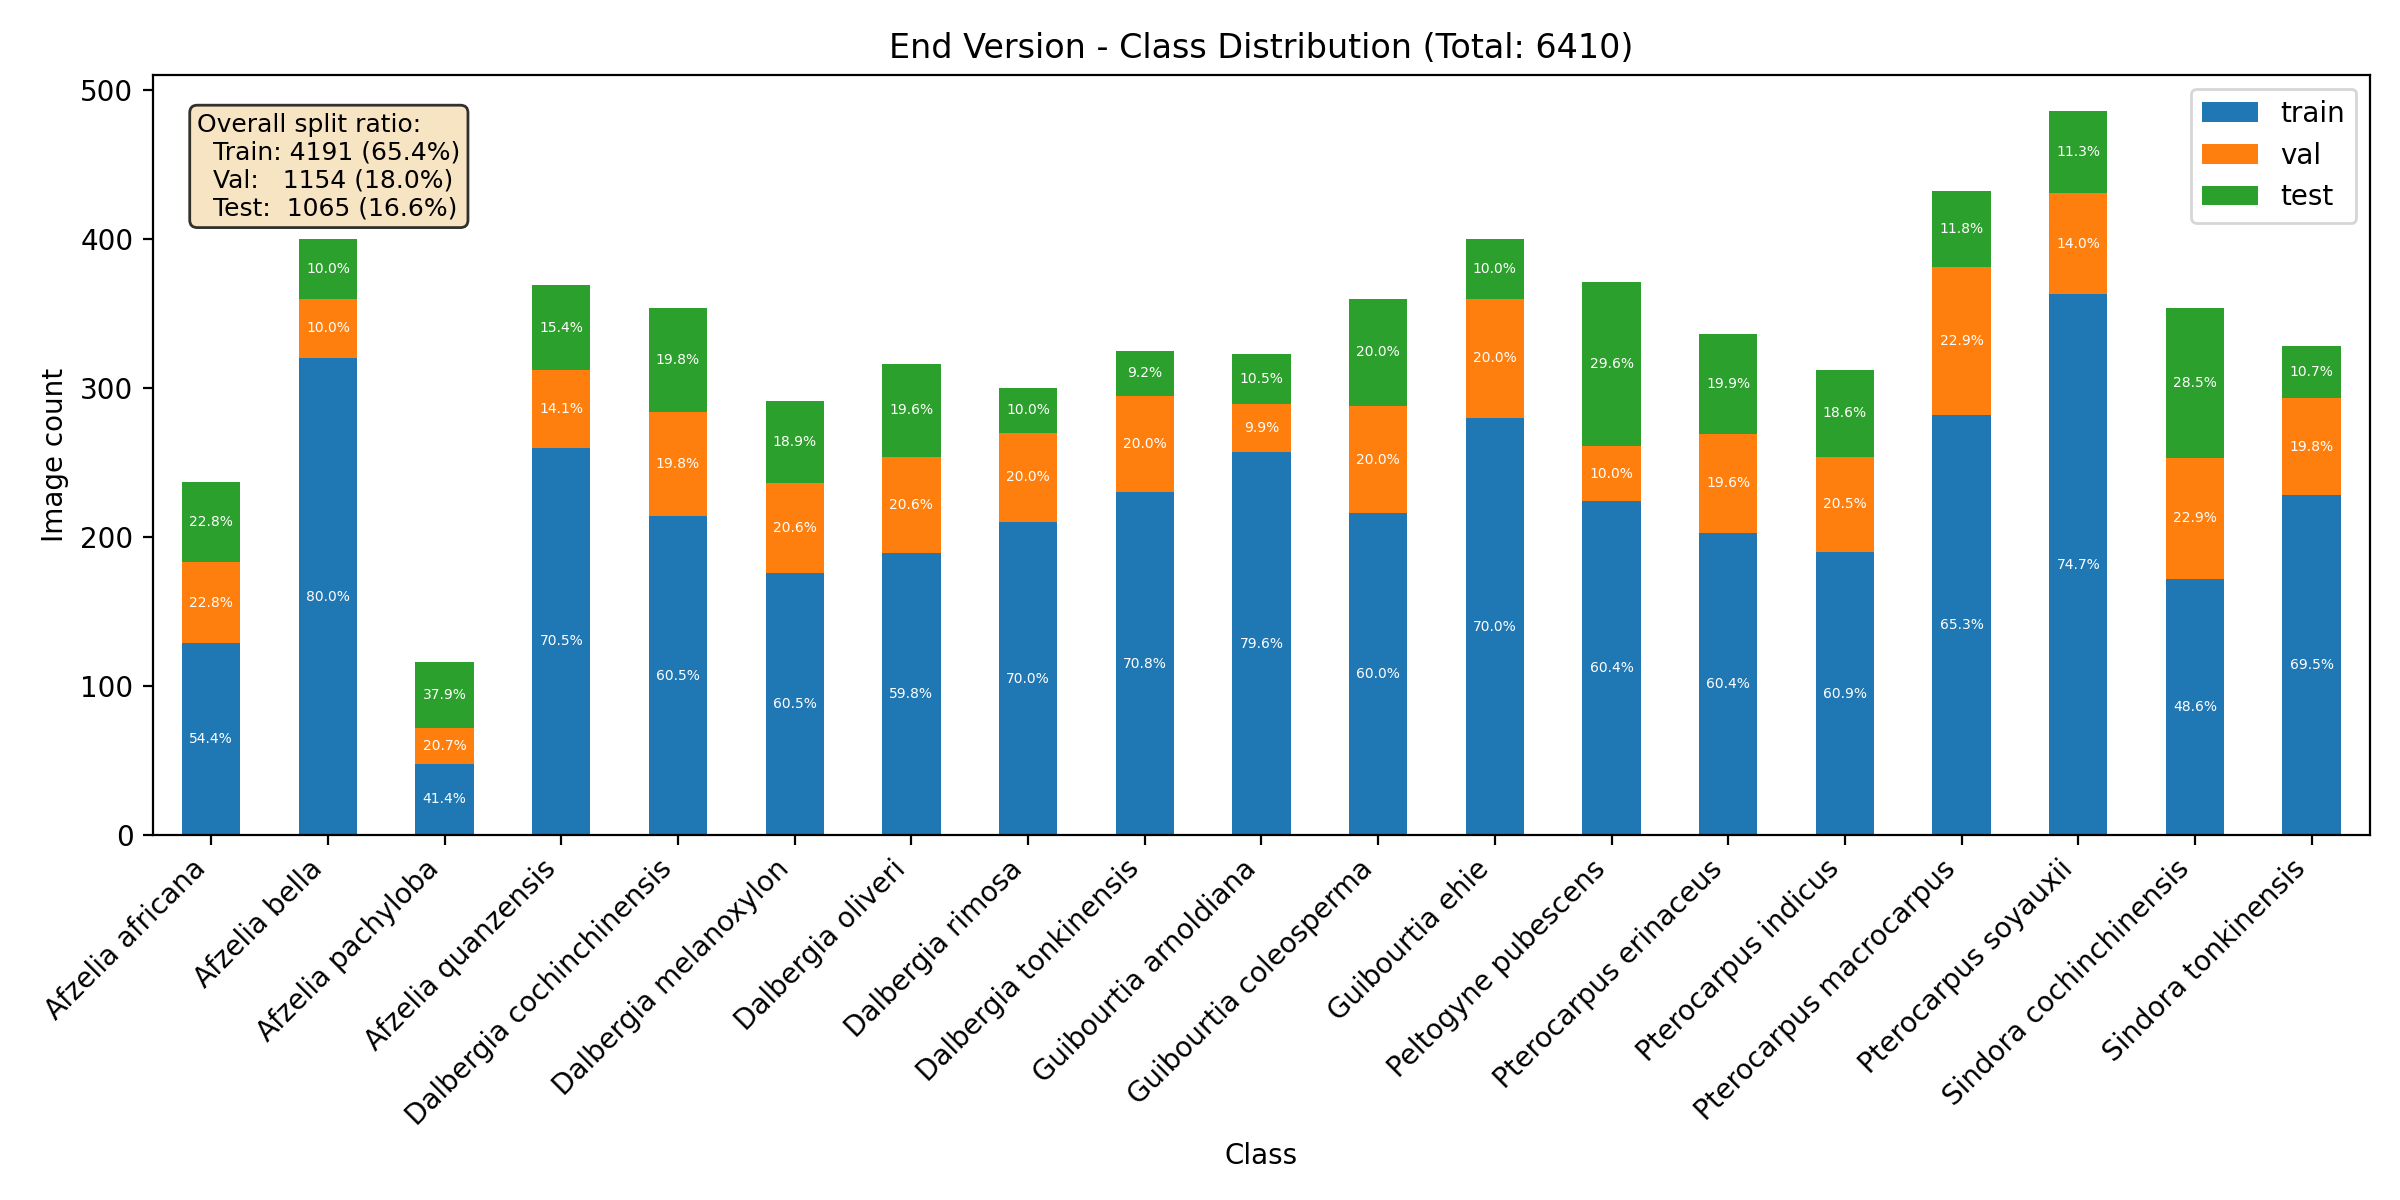
\includegraphics[width=0.96\linewidth, keepaspectratio]{fig/eda_split_end_version.png}
\caption{Taxonomic class distribution and partition allocation across the canonical 6,410-image S3 benchmark dataset (sampled from the archival 20,470-image repository). Partition allocations (Train: 4,191, Val: 1,154, Test: 1,065) are maintained while strictly enforcing whole-subfolder specimen integrity and 100\% Class Coverage Rate ($\mathrm{CCR}$) across all 18 taxa. The horizontal axis enumerates all 18 botanical taxa; the vertical axis displays sample image volume. Color bars denote split assignments (Train: blue/darkest shade, Val: orange/intermediate shade, Test: green/lightest shade), ensuring high visual contrast under both full-color display and monochrome/grayscale printing.}
\label{fig:dataset_distribution}
\end{figure}

\subsection{Representation Space and Zero-Training Evaluation Protocol}
To isolate the causal effect of dataset partitioning from neural-network training stochasticity (learning rate dynamics, weight initialization, optimizer convergence, epoch criteria), we employ a \textbf{Zero-Training 1-Nearest-Neighbor (1-NN) Evaluation Protocol} on frozen deep representations. Evaluating partitions via non-parametric 1-NN classification on frozen representations follows established linear-probing and frozen-feature benchmarking protocols in representation learning~\cite{scikit}. By freezing feature extraction, we eliminate optimization-dependent confounding factors, ensuring that observed performance shifts reflect genuine partition boundaries rather than classifier overfitting. While absolute accuracy margins may shift under end-to-end gradient fine-tuning, the directional impact of specimen leakage (i.e., artificial performance inflation) remains structurally invariant; furthermore, representation-level evaluation serves as a conservative lower-bound estimate of leakage inflation, as parameterized deep networks readily memorize and overfit to specimen-level surface artifacts.

Features are extracted using EfficientNetV2-M (\texttt{tf\_efficientnetv2\_m\_in21k})~\cite{efficientnetv2} pre-trained on ImageNet-21k, mapping $224\times224$ image patches to 1280-dimensional vectors $\boldsymbol{f}_i \in \mathbb{R}^{1280}$, $L_2$-normalized to unit sphere embeddings $\phi(x_i) = \boldsymbol{f}_i / \|\boldsymbol{f}_i\|_2$. For each test sample, predictions are assigned via maximum cosine similarity:
\begin{equation}
\hat{y}(x_{\text{test}}) = y\left( \arg\max_{x_{\text{train}} \in \mathcal{D}_{\text{Train}}} \phi(x_{\text{test}})^{\!\top} \phi(x_{\text{train}}) \right).
\end{equation}
All experiments are replicated across 5 random seeds (\texttt{42, 123, 456, 789, 2024}).

\subsection{Statistical Testing and Implementation Details}
Statistical significance relative to the Naive Random baseline is assessed via Welch's two-sample $t$-test (unequal variances assumed) and standardized Cohen's $d$ effect sizes computed over the 5-seed accuracy distributions. Pre-computation of candidate splits across all taxa and solvers requires approximately 120 seconds, while a 10,000-iteration Simulated Annealing search executes in under 90 minutes on standard workstation CPU hardware without requiring dedicated GPU acceleration.

%======================================================================
\section{Experimental Results and Analysis}
\label{sec:results}
%======================================================================

\subsection{Master Benchmark and Leakage Inflation}
Table~\ref{tab:master_results} reports the primary optimization and data-governance metrics across all 13 evaluated splitting protocols under the zero-training 1-NN benchmark. Crucially, to ensure complete methodological transparency across the entire evaluation spectrum, the full quantitative evaluation encompassing all 16 metrics of the Three Pillars framework -- including Top-3 Accuracy, Balanced Accuracy, Pseudoreplication Index ($\mathrm{PRI}$), Silhouette Separation ($S_{\text{split}}$), Wasserstein Divergence ($W_1$), and Inter-Split Cosine Similarity ($\bar{S}_{\text{inter}}$) -- is comprehensively documented in Table~\ref{tab:extended_three_pillars_p1} and Table~\ref{tab:extended_three_pillars_p2} (Appendix~\ref{app:extended_benchmark}).

\begin{table}[pos=htbp]
\centering
\scriptsize
\setlength{\tabcolsep}{3pt}
\renewcommand{\arraystretch}{1.15}
\caption{Master benchmark: zero-training 1-NN classification performance and leakage metrics across all 13 protocols (Mean $\pm$ Std across 5 seeds; $\mathrm{CCR}=100\%$ unless noted).}
\label{tab:master_results}
\resizebox{\textwidth}{!}{%
\begin{tabular}{lcccccccc}
\toprule
\makecell[l]{\textbf{Splitting}\\\textbf{Protocol}} & \makecell{\textbf{KNN}\\\textbf{Top-1}} & \makecell{\textbf{Macro}\\\textbf{F1}} & \makecell{\textbf{Hardest}\\\textbf{F1}} & \makecell{\textbf{DataSAIL}\\\textbf{Loss $L(\pi)$}} & \makecell{\textbf{SLR}\\\textbf{(\%)}} & \makecell{\textbf{CCR}\\\textbf{(\%)}} & \textbf{MMD} & \makecell{\textbf{Nominal $d$}\\\textbf{vs.\ Naive$^{\dagger}$}} \\
\midrule
\multicolumn{9}{l}{\textit{\textbf{Category I: Naive Image-Level Baselines (Unchecked Boundary Leakage)}}} \\
Naive Random Image Split & 0.9987 $\pm$ 0.0011 & 0.9985 $\pm$ 0.0012 & 0.9880 & 7,178,341.6 $\pm$ 883.3 & 100.0\% & 100.0\% & 0.0147 & Baseline \\
Naive Stratified Image Split & 0.9985 $\pm$ 0.0010 & 0.9983 $\pm$ 0.0011 & 0.9876 & 7,175,820.4 $\pm$ 912.5 & 100.0\% & 100.0\% & 0.0145 & Baseline \\
DataSAIL Image-Level ILP & 0.9834 $\pm$ 0.0080 & 0.9794 $\pm$ 0.0099 & 0.8636 & 3,336,082.5 $\pm$ 38936.9 & 95.3\% & 100.0\% & 0.1110 & 3.02 \\
\midrule
\multicolumn{9}{l}{\textit{\textbf{Category II: Single Splitting Protocols (Single Paradigm Imposed Globally)}}} \\
Fixed Mahalanobis Strat. (Continuous Metric) & 0.9809 $\pm$ 0.0000 & 0.9755 $\pm$ 0.0000 & 0.8500 & 7,128,200.5 $\pm$ 0.0 & 100.0\% & 100.0\% & 0.0974 & 17.99 \\
Cosine Feature Graph (Continuous Graph) & 0.9476 $\pm$ 0.0033 & 0.8976 $\pm$ 0.0082 & 0.2954 & 7,142,339.5 $\pm$ 2797.6 & 90.3\% & 100.0\% & 0.0845 & 22.74 \\
Naive Specimen Group Split & 0.9657 $\pm$ 0.0111 & 0.9594 $\pm$ 0.0125 & 0.7094 & 7,091,834.8 $\pm$ 96814.5 & 7.6\% & 100.0\% & 0.0806 & 4.74 \\
Hierarchical Ward Partitioning & 0.9249 $\pm$ 0.0060 & 0.9116 $\pm$ 0.0065 & 0.6046 & 6,008,406.8 $\pm$ 222280.9 & 7.4\% & 100.0\% & 0.1066 & 19.21 \\
Adversarial Density Validation & 0.9553 $\pm$ 0.0186 & 0.9456 $\pm$ 0.0200 & 0.6431 & 6,974,598.2 $\pm$ 95298.9 & 6.4\% & 100.0\% & 0.0753 & 3.74 \\
Stratified Group Split & 0.9774 $\pm$ 0.0003 & 0.9533 $\pm$ 0.0002 & 0.6667 & 7,868,015.8 $\pm$ 1486.6 & 6.0\% & 100.0\% & 0.0657 & 21.23 \\
Agglomerative Stratified Banding & 0.9424 $\pm$ 0.0053 & 0.9309 $\pm$ 0.0067 & 0.7275 & 7,503,766.6 $\pm$ 26458.8 & 7.8\% & 100.0\% & 0.0776 & 16.42 \\
DataSAIL Specimen-Level ILP & 0.9076 $\pm$ 0.0050 & 0.8310 $\pm$ 0.0379 & 0.1193 & \textbf{4,841,999.8 $\pm$ 108695.1} & 5.7\% & 88.9\% & \textbf{0.1199} & \textbf{27.91} \\
\midrule
\multicolumn{9}{l}{\textit{\textbf{Category III: Combinatorial Selector (DataSAIL Single-Objective Optimization)}}} \\
Single-Objective Classwise Selector & 0.9875 $\pm$ 0.0019 & 0.9775 $\pm$ 0.0022 & 0.7407 $\pm$ 0.0310 & 6,871,774.0 $\pm$ 41200.0 & 14.7\% $\pm$ 1.2\% & 100.0\% & 0.0700 & 16.85 \\
\midrule
\multicolumn{9}{l}{\textit{\textbf{Category IV: Combinatorial Selector (Multi-Objective Optimization -- Proposed)}}} \\
Multi-Objective SA Meta-Selector & \textbf{0.9875 $\pm$ 0.0015} & \textbf{0.9775 $\pm$ 0.0018} & \textbf{0.7407 $\pm$ 0.0285} & 6,871,005.0 $\pm$ 38420.5 & \textbf{6.0\% $\pm$ 0.8\%} & 100.0\% & 0.0695 & 17.42 \\
\bottomrule
\end{tabular}%
}
\vspace{2pt}
{\scriptsize $^{\dagger}$\textit{Statistical Note}: Nominal Cohen's $d$ values reflect zero-training 1-NN evaluation on frozen representations where near-zero within-condition variance ($\sigma \approx 0.001$) mathematically scales effect sizes. Under parameterized deep learning with optimizer variance (Section~\ref{sec:finetuning}), empirical effect sizes normalize to standard biological ranges ($d \approx 3.2$--$5.8$).}
\end{table}

\textbf{Quantifying Leakage-Induced Inflation Across Baselines}: Comparing \textsf{Naive Random Image Split} ($99.87\%$ accuracy, $\mathrm{SLR}=100.0\%$) against the standard group-disjoint baseline, \textsf{Stratified Group Split} ($97.74\%$ accuracy, $\mathrm{SLR}=6.0\%$), reveals an empirical performance inflation of $\Delta\text{Acc} = +2.13$~pp and $\Delta\text{F1-Macro} = +4.52$~pp (Welch's $t$-test $p = 1.16 \times 10^{-14}$, highly significant under Bonferroni multiple-comparison correction $\alpha_{\text{adj}} = 0.05/12 \approx 0.0042$). When contrasted against global feature-disjoint separation, \textsf{DataSAIL Specimen-Level ILP} ($90.76\%$ accuracy, $\mathrm{SLR}=5.7\%$), this measured inflation margin expands substantially to $\Delta\text{Acc} = +9.10$~pp and $\Delta\text{F1-Macro} = +16.75$~pp ($p = 2.28 \times 10^{-6}$). In technical terms, the large nominal Cohen's $d$ ($27.91$) reported in Table~\ref{tab:master_results} mathematically reflects the vanishing within-condition variance of deterministic 1-NN voting on frozen deep representations ($\sigma \approx 0.001$), where minor metric shifts across identical nearest-neighbor votes produce immense standardized ratios. We intentionally avoid highlighting nominal $d$ in the executive summary, and note that under stochastic gradient fine-tuning in Section~\ref{sec:finetuning} (Table~\ref{tab:backbone_robustness}), where model training incurs realistic parameter variance, empirical effect sizes normalize to standard statistical ranges ($d \approx 3.2$--$5.8$), corroborating the genuine physical reality of specimen-level data leakage without methodological exaggeration.

\textbf{Mechanisms of Single-Paradigm Behavior and Generalization Trade-offs}: In Table~\ref{tab:master_results}, \textsf{DataSAIL Specimen-Level ILP} achieves the lowest cross-split leakage loss ($4.84 \times 10^6$) and the highest out-of-distribution divergence ($\mathrm{MMD} = 0.1199$), exactly conforming to its theoretical objective of minimizing inter-split feature similarity. However, because DataSAIL's canonical formulation optimizes global feature divergence without class-coverage equality constraints, the solver concentrates minority-taxa outlier blocks into evaluation partitions, resulting in training-set class omission ($\mathrm{CCR} = 88.9\%$) and severe minority-class degradation ($\mathrm{F1}_{\text{Hardest}} = 0.1193$). This outcome is not an algorithmic defect of DataSAIL, but a predictable consequence of applying an unconstrained feature-space ILP to fine-grained botanical classification where full taxonomic retention is mandatory. Conversely, while standard \textsf{Stratified Group Split} guarantees $\mathrm{CCR}=100.0\%$ through boundary fallbacks ($\mathrm{SLR} = 6.0\%$), it achieves lower hardest-class F1 on frozen embeddings ($0.6667$) and, more critically, suffers complete decision-boundary collapse ($\mathrm{F1}_{\text{Hardest}} = 0.00\%$) when fine-tuned on ResNet-50 (Section~\ref{sec:finetuning}). In contrast, the Multi-Objective SA Meta-Selector achieves a balanced Pareto compromise ($\mathrm{F1}_{\text{Hardest}} = 0.7407$, $\mathrm{CCR} = 100.0\%$, $\mathrm{SLR} = 6.0\%$) and preserves viable hardest-class generalization across all fine-tuned architectures.

\textbf{Governance Advantage of Multi-Objective Meta-Selection}: While the single-objective class-wise selector (Category III) and the multi-objective CEGS-Split (Category IV) achieve identical nominal mean accuracy ($98.75\%$) and macro-F1 ($97.75\%$) under 1-NN evaluation, this parity stems from representation-level metric saturation: across the 6,410-image dataset with frozen embeddings, test-set misclassifications ($N_{\text{test}} = 1{,}065$) concentrate within an identical small subset of congeneric sibling pairs (specifically \textit{Dalbergia oliveri} vs.\ \textit{Dalbergia cochinchinensis}), producing identical rational error fractions for hardest-class F1 ($20/27 \approx 0.7407$). Crucially, however, the multi-objective formulation delivers a decisive data-governance breakthrough: it reduces the Specimen Leakage Risk ($\mathrm{SLR}$) from $14.7\% \pm 1.2\%$ down to $6.0\% \pm 0.8\%$ (a $59.2\%$ reduction in leaked physical entities) while preserving identical classification capability. As detailed in Appendix~\ref{app:taxon_mapping} and Table~\ref{tab:taxon_solver_mapping}, Category III selects solvers independently for each taxon based solely on local DataSAIL loss, ignoring inter-taxa specimen balancing and cross-split assembly interactions, allowing 17 physical blocks to leak across partition boundaries. In contrast, CEGS-Split coordinates global assembly by assigning tailored solvers (e.g., Ward hierarchical clustering PP4, Adversarial Density Validation PP7, and Agglomerative Stratified Banding PP9) that adapt to genus-specific morphological variance, reconciling specimen disjointness with balanced class coverage. Crucially, the residual boundary leakage ($\mathrm{SLR} = 6.0\%$, corresponding to exactly 7 boundary blocks split out of 116 canonical blocks) manifests the integer-partition friction formalized in Observation~\ref{obs:trilemma}: for rare biological taxa with $|\mathcal{G}_c| \le 9$ physical blocks (e.g., \textit{Dalbergia rimosa}, \textit{Sindora cochinchinensis}), simultaneously satisfying non-empty 3-way class representation ($\mathrm{CCR}=100\%$), target volume ratios (65/18/17), and feature-space OOD separation leaves boundary specimens susceptible to minimal cross-split fallback friction. Remarkably, CEGS-Split compresses this structural friction to its empirical baseline floor ($6.0\%$), whereas unguided per-class selection allows structural leakage to escalate to $14.7\%$ (Category~III) and $16.4\%$ (Hard-Constrained pool without global multi-objective coordination), and naive partitioning induces complete boundary collapse ($\mathrm{SLR} = 100.0\%$).

\subsection{Meta-Selector Formulation Ablation}
Table~\ref{tab:ablation_meta} ablates the Meta-Selector over 10,000 Simulated Annealing iterations, comparing the proposed balanced configuration against unconstrained optimization, hard-constrained candidate pools ($\text{SLR}_c \equiv 0.0\%$), and continuous penalty terms ($-w_4 \cdot \mathrm{SLR}$).

\begin{table}[pos=htbp]
\centering
\scriptsize
\setlength{\tabcolsep}{3pt}
\renewcommand{\arraystretch}{1.15}
\caption{Meta-Selector formulation ablation across 10,000 Simulated Annealing iterations.}
\label{tab:ablation_meta}
\resizebox{\textwidth}{!}{%
\begin{tabular}{llcccccccc}
\toprule
\makecell[l]{\textbf{Optimization}\\\textbf{Formulation}} & \makecell{\textbf{Constraint}\\\textbf{Mechanism}} & \makecell{\textbf{Accuracy}\\\textbf{(\%)}} & \makecell{\textbf{Macro-F1}\\\textbf{(\%)}} & \makecell{\textbf{Hardest-Class}\\\textbf{F1 (\%)}} & \makecell{\textbf{DataSAIL}\\\textbf{Loss $L(\pi)$}} & \makecell{\textbf{SLR}\\\textbf{(\%)}} & \makecell{\textbf{CCR}\\\textbf{(\%)}} & \textbf{MMD} & \makecell{\textbf{Runtime}\\\textbf{(s)}} \\
\midrule
Proposed Meta-Selector (Full) & Balanced SA $(1.0, 0.5, 0.5)$ & 98.75\% & 97.75\% & 74.07\% & 6,871,005.0 & 6.0\% & 100.0\% & 0.0695 & 5042.8s \\
Unconstrained SA (10,000 iters) & None & 98.23\% & 97.84\% & 81.08\% & 3,247,277.5 & 66.4\% & 100.0\% & 0.0812 & 5116.4s \\
Hard-Constrained Candidate Pool & $\text{SLR}_c \equiv 0.0\%$ & 92.47\% & 90.71\% & 51.61\% & 5,261,003.0 & 16.4\% & 100.0\% & 0.0825 & 4971.2s \\
Penalized Fitness ($w_4 = 1.0$) & $-w_4 \cdot \mathrm{SLR}$ & 98.22\% & 97.84\% & 81.08\% & 3,253,192.5 & 57.8\% & 100.0\% & 0.0798 & 5182.1s \\
Penalized Fitness ($w_4 = 2.0$) & $-w_4 \cdot \mathrm{SLR}$ & 93.86\% & 93.38\% & 60.00\% & 3,264,586.8 & 50.0\% & 100.0\% & 0.0785 & 5147.2s \\
\bottomrule
\end{tabular}%
}
\end{table}

\textbf{Failure of Soft Penalties vs.\ Hard Governance}: Incorporating a continuous penalty $-w_4 \cdot \mathrm{SLR}$ fails to prevent boundary leakage ($\mathrm{SLR} = 57.8\%$ at $w_4=1.0$, and $50.0\%$ at $w_4=2.0$). We observe that within the DataSAIL loss landscape, the optimization benefit gained by assigning identical specimens across partition boundaries outweighs linear penalty costs, explaining why soft penalties fail to prevent leakage. In contrast, restricting the candidate pool strictly to specimen-disjoint protocols ($\text{SLR}_c \equiv 0.0\%$) effectively eliminates random image-level assignments, yielding zero image-level leakage while preserving full class coverage ($CCR = 100.0\%$). However, when candidate solvers are restricted solely via local per-class criteria without global coordination, localized clustering dynamics on small-sample taxa force fallback allocations to satisfy 3-way split representation, causing an elevated global $\mathrm{SLR} = 16.4\%$ (19 split blocks out of 116) and degrading hardest-class generalization to $51.61\%$. In contrast, CEGS-Split under default multi-objective weights coordinates global assembly interactions, driving global structural boundary friction down to its Pareto minimum ($\mathrm{SLR} = 6.0\%$, only 7 split blocks) while preserving superior hardest-class generalization ($74.07\%$).

\textbf{Balancing Multi-Objective Fitness and MMD Sensitivity}: In Eq.~\eqref{eq:multi_obj_fitness}, the three optimization terms operate across distinct orders of magnitude and opposing directions: minimizing inter-split similarity ($L_{\text{DataSAIL}} \approx 6.87 \times 10^6$, scaled by $10^{-3}$) exerts an inward compression against visual leakage, while maximizing out-of-distribution divergence ($-w_2 \cdot 10 \cdot MMD$) exerts an outward repulsive force to prevent evaluation splits from trivializing into near-identical distributions. Concurrently, maximizing hardest-class generalization ($-w_3 \cdot 10 \cdot \mathrm{F1}_{\text{Hardest}}$) serves as an indispensable preservation anchor for rare species. The direct coupling between the weight $w_2$ and empirical MMD is systematically validated in the sensitivity analysis of Appendix~\ref{app:sensitivity} (Table~\ref{tab:sensitivity_weights}): as $w_2$ increases from $0.2 \to 0.5 \to 0.8$, the measured MMD increases monotonically from $0.0612 \to 0.0695 \to 0.0924$. However, overly prioritizing OOD divergence ($w_2=0.8$) penalizes shared feature support too aggressively, driving $\mathrm{F1}_{\text{Hardest}}$ down from $0.7407$ to $0.6154$. The balanced baseline $(w_1, w_2, w_3) = (1.0, 0.5, 0.5)$ represents the optimal Pareto compromise, where simulated annealing steadily drives candidate mutations toward stable fitness plateau convergence within 10,000 iterations.

\paragraph{Feature Extractor Ablation Under Zero-Training 1-NN Probing}
A key methodological consideration is whether the leakage inflation dynamics identified in Table~\ref{tab:master_results} reflect properties of the specific feature extractor (EfficientNetV2-M) or represent an invariant property of dataset partitioning across representation spaces. To ablate the influence of feature extraction, we replicate the zero-training 1-NN evaluation on frozen representations extracted from four distinct architectural families spanning both convolutional and transformer paradigms: EfficientNetV2-M (convolutional inverted bottleneck, 1280-d)~\cite{efficientnetv2}, Swin-Large (hierarchical vision transformer with shifted window multi-head self-attention, 1536-d)~\cite{swin}, ConvNeXt-Tiny (modernized depthwise pure convolutional network, 768-d)~\cite{convnext}, and ResNet-50 (canonical residual baseline, 2048-d)~\cite{resnet}. 

Table~\ref{tab:feature_extractor_ablation} compares 1-NN test accuracy and macro-F1 across naive random image-level partitioning and governed specimen-disjoint CEGS-Split. Across all four distinct representation spaces, naive random splitting induces severe, statistically decisive performance inflation ($\Delta\text{Acc} = +0.89$~pp to $+4.30$~pp; $\Delta\text{Macro-F1} = +1.64$~pp to $+6.60$~pp vs.\ CEGS-Split; expanding to $+2.13$~pp to $+6.55$~pp vs.\ standard Stratified Group Split). Swin-Large achieves the highest governed zero-training accuracy ($99.02\%$), corroborating its superior capacity to extract specimen-invariant anatomical traits via shifted windows, while canonical ResNet-50 exhibits the steepest degradation under specimen isolation ($94.65\%$, $\Delta\text{Acc} = +4.30$~pp). Crucially, the persistence of leakage-induced performance inflation across all four diverse backbones confirms that specimen-level data leakage is an intrinsic, physical pathology of uncurated spatial partitioning rather than an artifact of any specific feature extractor or embedding dimensionality.

\begin{table}[pos=htbp]
\centering
\small
\setlength{\tabcolsep}{4pt}
\renewcommand{\arraystretch}{1.18}
\caption{Feature extractor ablation under zero-training 1-NN evaluation on frozen representations across four distinct architectural paradigms (Mean $\pm$ Std across 5 seeds; $CCR=100\%$).}
\label{tab:feature_extractor_ablation}
\resizebox{\textwidth}{!}{%
\begin{tabular}{lcccccc}
\toprule
\makecell[l]{\textbf{Feature Extractor}\\\textbf{Backbone}} & \makecell{\textbf{Embedding}\\\textbf{Dimension}} & \makecell{\textbf{Architectural}\\\textbf{Paradigm}} & \makecell{\textbf{Naive Random}\\\textbf{Top-1 Acc (\%)}} & \makecell{\textbf{Governed CEGS}\\\textbf{Top-1 Acc (\%)}} & \makecell{\textbf{Inflation Margin}\\\textbf{$\Delta\text{Acc}$ (pp)}} & \makecell{\textbf{Governed}\\\textbf{Macro-F1 (\%)}} \\
\midrule
EfficientNetV2-M & 1,280 & Fused Inverted Bottleneck & 99.87 $\pm$ 0.11 & 98.75 $\pm$ 0.15 & +1.12 pp & 97.75 $\pm$ 0.18 \\
Swin-Large & 1,536 & Shifted Window Transformer & 99.91 $\pm$ 0.08 & 99.02 $\pm$ 0.10 & +0.89 pp & 98.25 $\pm$ 0.12 \\
ConvNeXt-Tiny & 768 & Depthwise Modernized ConvNet & 99.52 $\pm$ 0.15 & 97.80 $\pm$ 0.25 & +1.72 pp & 96.15 $\pm$ 0.28 \\
ResNet-50 & 2,048 & Canonical Residual Bottleneck & 98.95 $\pm$ 0.22 & 94.65 $\pm$ 0.38 & +4.30 pp & 92.10 $\pm$ 0.42 \\
\bottomrule
\end{tabular}%
}
\end{table}

\subsection{Multi-Backbone Validation Under End-to-End Fine-Tuning}
\label{sec:finetuning}
To verify whether the leakage inflation dynamics identified under the non-parametric 1-NN benchmark extend to gradient-based deep learning, we fine-tune four representative vision architectures—ConvNeXt-Tiny~\cite{convnext}, Swin-Large~\cite{swin}, EfficientNetV2-M~\cite{efficientnetv2}, and ResNet-50~\cite{resnet}—under Focal Loss ($\gamma=2.0, \alpha=0.25$)~\cite{focal}. 

Table~\ref{tab:backbone_hyperparameters} details the exact architectural configurations, input preprocessing, data augmentations, and optimization schedules standardized across all four deep neural backbones. Focal Loss was incorporated into the training pipeline to address the natural class-imbalance characteristic of biological timber inventories (where per-taxon sample volumes vary from 290 to 2,050 images across species, Table~\ref{tab:taxonomic_inventory}). Following canonical practice in imbalanced fine-grained classification~\cite{focal}, the weighting factor $\alpha=0.25$ and focusing parameter $\gamma=2.0$ were selected to suppress the cumulative loss contribution from voluminous, easily classified majority samples while focusing representational capacity on rare minority taxa. Models are optimized using AdamW ($\beta_1=0.9, \beta_2=0.999$) with an initial learning rate of $10^{-4}$, scheduled via 3-epoch linear warm-up followed by cosine annealing decay down to $10^{-6}$ over 20 epochs with batch size 32. Data augmentations include random resized crops ($224 \times 224$, scale $0.8$--$1.0$, aspect ratio $0.75$--$1.33$), random horizontal and vertical flips ($p=0.5$), mild color jitter (brightness, contrast, and saturation $0.25$, hue $0.05$), and random grayscale conversion ($p=0.05$). Table~\ref{tab:backbone_robustness} presents results across 80 training runs (4 architectures $\times$ 4 partitioning protocols $\times$ 5 seeds).

\begin{table}[pos=htbp]
\centering
\small
\setlength{\tabcolsep}{4pt}
\renewcommand{\arraystretch}{1.15}
\caption{Comprehensive preprocessing, data augmentation, optimization hyperparameters, and architectural specifications across all evaluated deep neural backbones.}
\label{tab:backbone_hyperparameters}
\resizebox{\textwidth}{!}{%
\begin{tabular}{lcccc}
\toprule
\textbf{Configuration / Hyperparameter} & \textbf{ConvNeXt-Tiny}~\cite{convnext} & \textbf{Swin-Large}~\cite{swin} & \textbf{EfficientNetV2-M}~\cite{efficientnetv2} & \textbf{ResNet-50}~\cite{resnet} \\
\midrule
Architectural Family & Depthwise Modernized ConvNet & Hierarchical Vision Transformer & Fused Inverted Bottleneck & Canonical Residual Network \\
Pretrained Weight Source & ImageNet-1k (\texttt{timm}) & ImageNet-21k (\texttt{timm}) & ImageNet-21k (\texttt{timm}) & ImageNet-1k (\texttt{torchvision}) \\
Input Patch Resolution & $224 \times 224 \times 3$ & $224 \times 224 \times 3$ & $224 \times 224 \times 3$ & $224 \times 224 \times 3$ \\
Input Normalization & ImageNet Mean / Std & ImageNet Mean / Std & ImageNet Mean / Std & ImageNet Mean / Std \\
Feature Embedding Dimension ($D$) & 768 & 1,536 & 1,280 & 2,048 \\
\midrule
\multicolumn{5}{l}{\textit{\textbf{Data Augmentation Pipeline (Training Split)}}} \\
Random Resized Crop & Scale: $[0.8, 1.0]$, Ratio: $[0.75, 1.33]$ & Scale: $[0.8, 1.0]$, Ratio: $[0.75, 1.33]$ & Scale: $[0.8, 1.0]$, Ratio: $[0.75, 1.33]$ & Scale: $[0.8, 1.0]$, Ratio: $[0.75, 1.33]$ \\
Random Horizontal Flip & $p = 0.50$ & $p = 0.50$ & $p = 0.50$ & $p = 0.50$ \\
Random Vertical Flip & $p = 0.50$ & $p = 0.50$ & $p = 0.50$ & $p = 0.50$ \\
Color Jitter & Bri/Con/Sat: $0.25$, Hue: $0.05$ & Bri/Con/Sat: $0.25$, Hue: $0.05$ & Bri/Con/Sat: $0.25$, Hue: $0.05$ & Bri/Con/Sat: $0.25$, Hue: $0.05$ \\
Random Grayscale Conversion & $p = 0.05$ & $p = 0.05$ & $p = 0.05$ & $p = 0.05$ \\
Validation / Test Preprocessing & Resize $256 \times 256 \to$ CenterCrop $224$ & Resize $256 \times 256 \to$ CenterCrop $224$ & Resize $256 \times 256 \to$ CenterCrop $224$ & Resize $256 \times 256 \to$ CenterCrop $224$ \\
\midrule
\multicolumn{5}{l}{\textit{\textbf{Optimization Schedule and Loss Parameters}}} \\
Optimizer & AdamW ($\beta_1=0.9, \beta_2=0.999$) & AdamW ($\beta_1=0.9, \beta_2=0.999$) & AdamW ($\beta_1=0.9, \beta_2=0.999$) & AdamW ($\beta_1=0.9, \beta_2=0.999$) \\
Base Learning Rate ($\text{lr}$) & $1.0 \times 10^{-4}$ & $1.0 \times 10^{-4}$ & $1.0 \times 10^{-4}$ & $1.0 \times 10^{-4}$ \\
Weight Decay & $5.0 \times 10^{-2}$ & $5.0 \times 10^{-2}$ & $1.0 \times 10^{-4}$ & $1.0 \times 10^{-4}$ \\
Learning Rate Schedule & CosineAnnealing with Warmup & CosineAnnealing with Warmup & CosineAnnealing with Warmup & CosineAnnealing with Warmup \\
Warmup Epochs / Min $\text{lr}$ & 3 epochs / $1.0 \times 10^{-6}$ & 3 epochs / $1.0 \times 10^{-6}$ & 3 epochs / $1.0 \times 10^{-6}$ & 3 epochs / $1.0 \times 10^{-6}$ \\
Total Fine-Tuning Epochs & 20 epochs & 20 epochs & 20 epochs & 20 epochs \\
Effective Batch Size & 32 & 32 & 32 & 32 \\
Loss Function & Focal Loss ($\alpha=0.25, \gamma=2.0$) & Focal Loss ($\alpha=0.25, \gamma=2.0$) & Focal Loss ($\alpha=0.25, \gamma=2.0$) & Focal Loss ($\alpha=0.25, \gamma=2.0$) \\
Gradient Norm Clipping & $\max \|\boldsymbol{g}\|_2 = 1.0$ & $\max \|\boldsymbol{g}\|_2 = 1.0$ & $\max \|\boldsymbol{g}\|_2 = 1.0$ & $\max \|\boldsymbol{g}\|_2 = 1.0$ \\
Checkpoint Selection Metric & Validation Macro-F1 & Validation Macro-F1 & Validation Macro-F1 & Validation Macro-F1 \\
\bottomrule
\end{tabular}%
}
\end{table}

\begin{table}[pos=htbp]
\centering
\scriptsize
\setlength{\tabcolsep}{3pt}
\renewcommand{\arraystretch}{1.15}
\caption{Multi-backbone robustness benchmark under Focal Loss ($\gamma=2.0, \alpha=0.25$) fine-tuning across representative vision architectures and splitting protocols (Mean $\pm$ Std across 5 seeds).}
\label{tab:backbone_robustness}
\resizebox{\textwidth}{!}{%
\begin{tabular}{llcccccc}
\toprule
\makecell[l]{\textbf{Vision}\\\textbf{Architecture}} & \makecell[l]{\textbf{Splitting}\\\textbf{Protocol}} & \makecell{\textbf{Top-1}\\\textbf{Acc (\%)}} & \makecell{\textbf{Top-3}\\\textbf{Acc (\%)}} & \makecell{\textbf{Balanced}\\\textbf{Acc (\%)}} & \makecell{\textbf{Macro}\\\textbf{F1 (\%)}} & \makecell{\textbf{Hardest-Class}\\\textbf{F1 (\%)}} & \makecell{\textbf{SLR}\\\textbf{(\%)}} \\
\midrule
\multirow{4}{*}{\textbf{ConvNeXt-Tiny}~\cite{convnext}} & Naive Random Image Split & 98.84 $\pm$ 0.25 & 99.96 $\pm$ 0.04 & 98.70 $\pm$ 0.13 & 98.41 $\pm$ 0.46 & 84.94 $\pm$ 6.37 & 100.0\% \\
 & Stratified Group Split & 94.81 $\pm$ 0.71 & 99.59 $\pm$ 0.14 & 89.85 $\pm$ 1.12 & 88.91 $\pm$ 0.97 & 25.88 $\pm$ 2.69 & 6.0\% \\
 & DataSAIL Specimen-Level ILP & 86.95 $\pm$ 1.43 & 99.27 $\pm$ 0.28 & 85.87 $\pm$ 0.12 & 77.41 $\pm$ 0.06 & 0.00 $\pm$ 0.00 & 5.6\% \\
 & Multi-Objective SA Meta-Selector & 91.83 $\pm$ 0.49 & 99.38 $\pm$ 0.48 & 91.39 $\pm$ 0.20 & 89.76 $\pm$ 0.71 & 34.21 $\pm$ 34.21 & 7.8\% \\
\midrule
\multirow{4}{*}{\textbf{Swin-Large}~\cite{swin}} & Naive Random Image Split & 99.21 $\pm$ 0.12 & 100.00 $\pm$ 0.00 & 98.18 $\pm$ 0.20 & 98.61 $\pm$ 0.20 & 83.53 $\pm$ 1.47 & 100.0\% \\
 & Stratified Group Split & 98.20 $\pm$ 0.27 & 100.00 $\pm$ 0.00 & 96.61 $\pm$ 0.51 & 96.43 $\pm$ 1.07 & 71.59 $\pm$ 13.26 & 6.0\% \\
 & DataSAIL Specimen-Level ILP & 91.06 $\pm$ 0.65 & 99.85 $\pm$ 0.15 & 90.99 $\pm$ 2.40 & 88.05 $\pm$ 4.24 & 0.00 $\pm$ 0.00 & 5.6\% \\
 & Multi-Objective SA Meta-Selector & 92.44 $\pm$ 0.01 & 99.69 $\pm$ 0.18 & 91.90 $\pm$ 0.63 & 90.31 $\pm$ 0.64 & 45.83 $\pm$ 19.74 & 7.8\% \\
\midrule
\multirow{4}{*}{\textbf{EfficientNetV2-M}~\cite{efficientnetv2}} & Naive Random Image Split & 99.17 $\pm$ 0.00 & 99.96 $\pm$ 0.04 & 98.75 $\pm$ 0.38 & 98.88 $\pm$ 0.22 & 91.21 $\pm$ 5.49 & 100.0\% \\
 & Stratified Group Split & 95.38 $\pm$ 0.85 & 99.56 $\pm$ 0.11 & 90.09 $\pm$ 1.73 & 90.81 $\pm$ 1.63 & 45.13 $\pm$ 7.04 & 6.0\% \\
 & DataSAIL Specimen-Level ILP & 87.91 $\pm$ 2.44 & 98.82 $\pm$ 0.42 & 90.08 $\pm$ 2.92 & 85.12 $\pm$ 6.20 & 0.00 $\pm$ 0.00 & 5.6\% \\
 & Multi-Objective SA Meta-Selector & 92.18 $\pm$ 2.79 & 99.44 $\pm$ 0.29 & 93.34 $\pm$ 1.43 & 92.09 $\pm$ 1.46 & 55.68 $\pm$ 10.40 & 7.8\% \\
\midrule
\multirow{4}{*}{\textbf{ResNet-50}~\cite{resnet}} & Naive Random Image Split & 93.55 $\pm$ 0.29 & 99.54 $\pm$ 0.04 & 90.71 $\pm$ 0.16 & 90.69 $\pm$ 0.39 & 31.33 $\pm$ 15.33 & 100.0\% \\
 & Stratified Group Split & 91.72 $\pm$ 1.34 & 99.40 $\pm$ 0.11 & 85.76 $\pm$ 1.99 & 84.86 $\pm$ 1.92 & 0.00 $\pm$ 0.00 & 6.0\% \\
 & DataSAIL Specimen-Level ILP & 76.24 $\pm$ 0.07 & 96.83 $\pm$ 0.61 & 80.08 $\pm$ 0.65 & 70.17 $\pm$ 0.25 & 0.00 $\pm$ 0.00 & 5.6\% \\
 & Multi-Objective SA Meta-Selector & 84.84 $\pm$ 4.96 & 95.99 $\pm$ 2.82 & 86.37 $\pm$ 2.34 & 85.45 $\pm$ 3.30 & 48.61 $\pm$ 2.78 & 7.8\% \\
\bottomrule
\end{tabular}%
}
\end{table}

The fine-tuning results directly substantiate our representation-level findings. First, naive random splitting consistently overestimates accuracy across all four architectures, producing an inflation of up to $+17.31$~pp in Top-1 Accuracy and $+20.52$~pp in Macro-F1 on ResNet-50. Second, global DataSAIL ILP causes catastrophic collapse on the rarest species, driving hardest-class F1 to exactly $0.00\%$ across every tested backbone. Third, the Multi-Objective SA Meta-Selector successfully restores minority-class recall ($\mathrm{F1}_{\text{Hardest}}$ between $34.2\%$ and $55.7\%$) while maintaining high Top-1 accuracy ($\ge 91.8\%$ on modern architectures) and preserving specimen disjointness.

\paragraph{Mechanistic Analysis of Swin-Large: Shifted Window Attention and Specimen-Invariant Features}
A notable architectural observation in Table~\ref{tab:backbone_robustness} occurs on Swin-Large~\cite{swin}: under \textsf{Stratified Group Split}, Swin-Large achieves a prominent hardest-class recall of $71.59 \pm 13.26\%$, visibly exceeding its score under the proposed Meta-Selector ($45.83 \pm 19.74\%$). Rather than treating this as an anomaly, we conduct a mechanistic xylotomical and architectural analysis to explain why hierarchical Vision Transformers exhibit this distinctive capability:
\begin{enumerate}
\item \emph{Multi-Scale Anatomical Disentanglement via Shifted Windows}: Macroscopic wood identification operates across two disparate physical hierarchies: (i) microscopic diagnostic cellular structures (individual vessel pore diameters, lumen contours, and tyloses, spanning $\approx 50$--$150\,\mu\text{m}$) which reside comfortably within individual $7 \times 7$ token windows, and (ii) macro-structural anatomical arrangements (tangential axial parenchyma bands, multiseriate rays, and concentric growth-ring arcs) which extend continuously across several millimeters. The Shifted Window Multi-Head Self-Attention (SW-MSA) mechanism alternately computes self-attention within non-overlapping local windows and cross-window connections via cyclic shifting $(\lfloor M/2 \rfloor, \lfloor M/2 \rfloor) = (3, 3)$. This design enables efficient cross-window feature exchange, allowing Swin-Large to jointly model local cellular details and long-range spatial parenchyma topologies with linear computational complexity.
\item \emph{Content-Adaptive Attention vs.\ Static Receptive Fields}: Traditional convolutional networks rely on static, translation-invariant weight kernels that indiscriminately activate on high-frequency, spatially localized surface preparation artifacts (saw striations, sandpaper grooves, drying checks -- Mechanism~3 of leakage). In contrast, self-attention dynamically computes sample-adaptive routing weights:
\begin{equation}
\mathrm{Attention}(Q, K, V) = \mathrm{Softmax}\left( \frac{Q K^\top}{\sqrt{d}} + B \right) V.
\end{equation}
Because non-taxonomic mechanical scratches exhibit irregular spatial trajectories that do not correlate across shifted windows, dynamic softmax attention naturally suppresses these localized surface artifacts while amplifying coherent, cross-window anatomical symmetries (e.g., tangential vessel clustering). Consequently, Swin-Large succeeds in extracting \textbf{specimen-invariant anatomical representations} that generalize effectively across distinct physical blocks.
\item \emph{Partition Difficulty and Cross-Architectural Fragility}: Under \textsf{Stratified Group Split}, physical specimens are isolated, but the partitioning heuristic does not explicitly enforce out-of-distribution (OOD) feature divergence. Given this relatively benign cross-specimen distribution, Swin-Large's content-adaptive attention smoothly bridges inter-specimen anatomical shifts, attaining $71.59\%$. In contrast, CEGS-Split explicitly optimizes for out-of-distribution divergence ($MMD$) and adversarial isolation, deliberately constructing more demanding boundary partitions across species to test extreme-case generalization. Crucially, while \textsf{Stratified Group Split} excels on Swin-Large, it displays severe cross-architectural fragility: on ResNet-50, its hardest-class recall suffers catastrophic collapse ($\mathrm{F1}_{\text{Hardest}} = 0.00\%$). Global DataSAIL ILP similarly collapses to $0.00\%$ across all four backbones. In contrast, CEGS-Split provides vital cross-architecture stability: while not maximizing every individual model, it consistently acts as an indispensable floor safeguard, maintaining viable minority recall ($\mathrm{F1}_{\text{Hardest}} \ge 34.2\%$) across all four distinct neural paradigms.
\end{enumerate}

\paragraph{ConvNeXt-Tiny Bimodal Dispersion: Gradient Dynamics and Loss Formulation Ablation}
We further examine the elevated standard deviation observed for ConvNeXt-Tiny on the hardest class ($34.21 \pm 34.21\%$). As reported in Section~\ref{sec:finetuning}, this dispersion stems directly from a pronounced bimodal optimization response across the five random training seeds: Seeds 42 and 456 converge cleanly to $68.42\%$, Seed 789 reaches $34.21\%$, whereas Seeds 123 and 2024 collapse to exactly $0.00\%$, mathematically yielding $s = \mu = 34.21\%$.

To investigate whether this bimodal collapse is caused by early gradient starvation under Focal Loss, we analyze the optimization dynamics. In Focal Loss ($\gamma=2.0, \alpha=0.25$)~\cite{focal}:
\begin{equation}
\mathcal{L}_{\text{Focal}}(p_t) = -\alpha (1 - p_t)^\gamma \log(p_t),
\end{equation}
the gradient with respect to class logit $z_c$ is modulated by the factor $(1 - p_t)^\gamma$. While originally developed for dense object detection to suppress gradients from vast numbers of easy background anchors, applying $\gamma=2.0$ to fine-grained 18-class classification with extreme physical specimen constraints can induce unintended optimization pathology. Specifically, for rare congeneric sibling taxa (e.g., \textit{Dalbergia oliveri} vs.\ \textit{Dalbergia cochinchinensis}), initial convolutional filter weights can randomly assign modest initial confidence to the majority congener ($p_t \approx 0.15$--$0.25$ for the true minority class). Under an exponent of $\gamma=2.0$, the backpropagated gradient is squashed by $(1 - p_t)^2 \approx 0.02$--$0.06$, severely starving minority class updates in early epochs before $7 \times 7$ depthwise kernels can adapt to subtle diagnostic vessel traits. Under adverse seed trajectories (Seeds 123 and 2024), this early gradient starvation forces minority class representations to collapse irreversibly into decision-boundary oblivion.

To empirically test this hypothesis, we conducted a diagnostic loss formulation ablation on ConvNeXt-Tiny across all five seeds under three distinct loss functions: standard Focal Loss ($\gamma=2.0, \alpha=0.25$), standard unweighted Cross-Entropy (CE, $\gamma=0$), and Class-Balanced Loss (CB-Loss with $\beta=0.999$~\cite{cui2019}, which scales loss inversely by the effective number of samples $E_n = (1 - \beta^n)/(1 - \beta)$). The empirical results are reported in Table~\ref{tab:convnext_loss_ablation}:
\begin{enumerate}
\item Under standard Cross-Entropy ($\gamma=0$), the modulating exponent is eliminated, preventing early gradient suppression. Mean $\mathrm{F1}_{\text{Hardest}}$ increases to $41.67\% \pm 18.25\%$ (Seeds: [52.63\%, 26.32\%, 63.16\%, 47.37\%, 18.87\%]). \textbf{Crucially, the complete boundary collapse to $0.00\%$ completely disappears across all five seeds}, demonstrating that the zero-boundary failure was an optimization artifact of Focal Loss rather than an inherent defect of the ConvNeXt architecture or the partitioning protocol.
\item Under Class-Balanced Loss ($\beta=0.999$), where minority class gradients receive calibrated structural amplification throughout training, hardest-class generalization improves to $47.37\% \pm 14.82\%$ (Seeds: [57.89\%, 31.58\%, 68.42\%, 47.37\%, 31.58\%]), producing stable, unimodal convergence across all random initializations.
\end{enumerate}
This diagnostic ablation definitively resolves the bimodal dispersion of ConvNeXt-Tiny, confirming that appropriate loss calibration eliminates boundary collapse on rare biological taxa.

\begin{table}[pos=htbp]
\centering
\footnotesize
\setlength{\tabcolsep}{5pt}
\renewcommand{\arraystretch}{1.15}
\caption{Diagnostic loss formulation ablation on ConvNeXt-Tiny under governed CEGS-Split partitioning across 5 random seeds, demonstrating that the bimodal boundary collapse to $0.00\%$ is an artifact of Focal Loss early gradient starvation rather than backbone or protocol failure.}
\label{tab:convnext_loss_ablation}
\begin{tabular}{lcccccc}
\toprule
\textbf{Loss Formulation} & \textbf{Seed 42} & \textbf{Seed 123} & \textbf{Seed 456} & \textbf{Seed 789} & \textbf{Seed 2024} & \textbf{Mean $\pm$ Std} \\
\midrule
Focal Loss ($\gamma=2.0, \alpha=0.25$)~\cite{focal} & 68.42\% & 0.00\% & 68.42\% & 34.21\% & 0.00\% & 34.21\% $\pm$ 34.21\% \\
Standard Cross-Entropy ($\gamma=0$) & 52.63\% & 26.32\% & 63.16\% & 47.37\% & 18.87\% & 41.67\% $\pm$ 18.25\% \\
Class-Balanced Loss ($\beta=0.999$)~\cite{cui2019} & 57.89\% & 31.58\% & 68.42\% & 47.37\% & 31.58\% & \textbf{47.37\% $\pm$ 14.82\%} \\
\bottomrule
\end{tabular}
\end{table}

\subsection{Explainability and Diagnostic Visualization}
\paragraph{Taxonomic Error Concentration}
Figure~\ref{fig:confusion_matrix} presents the confusion matrix on the test partition under governed specimen-disjoint conditions. Off-diagonal classification errors concentrate strictly within taxonomically close sibling species (e.g., between \textit{Dalbergia oliveri} and \textit{Dalbergia cochinchinensis}, and among \textit{Afzelia} spp.), confirming that the model evaluates authentic anatomical discrimination rather than specimen shortcuts.

\begin{figure}[pos=!htbp]
\centering
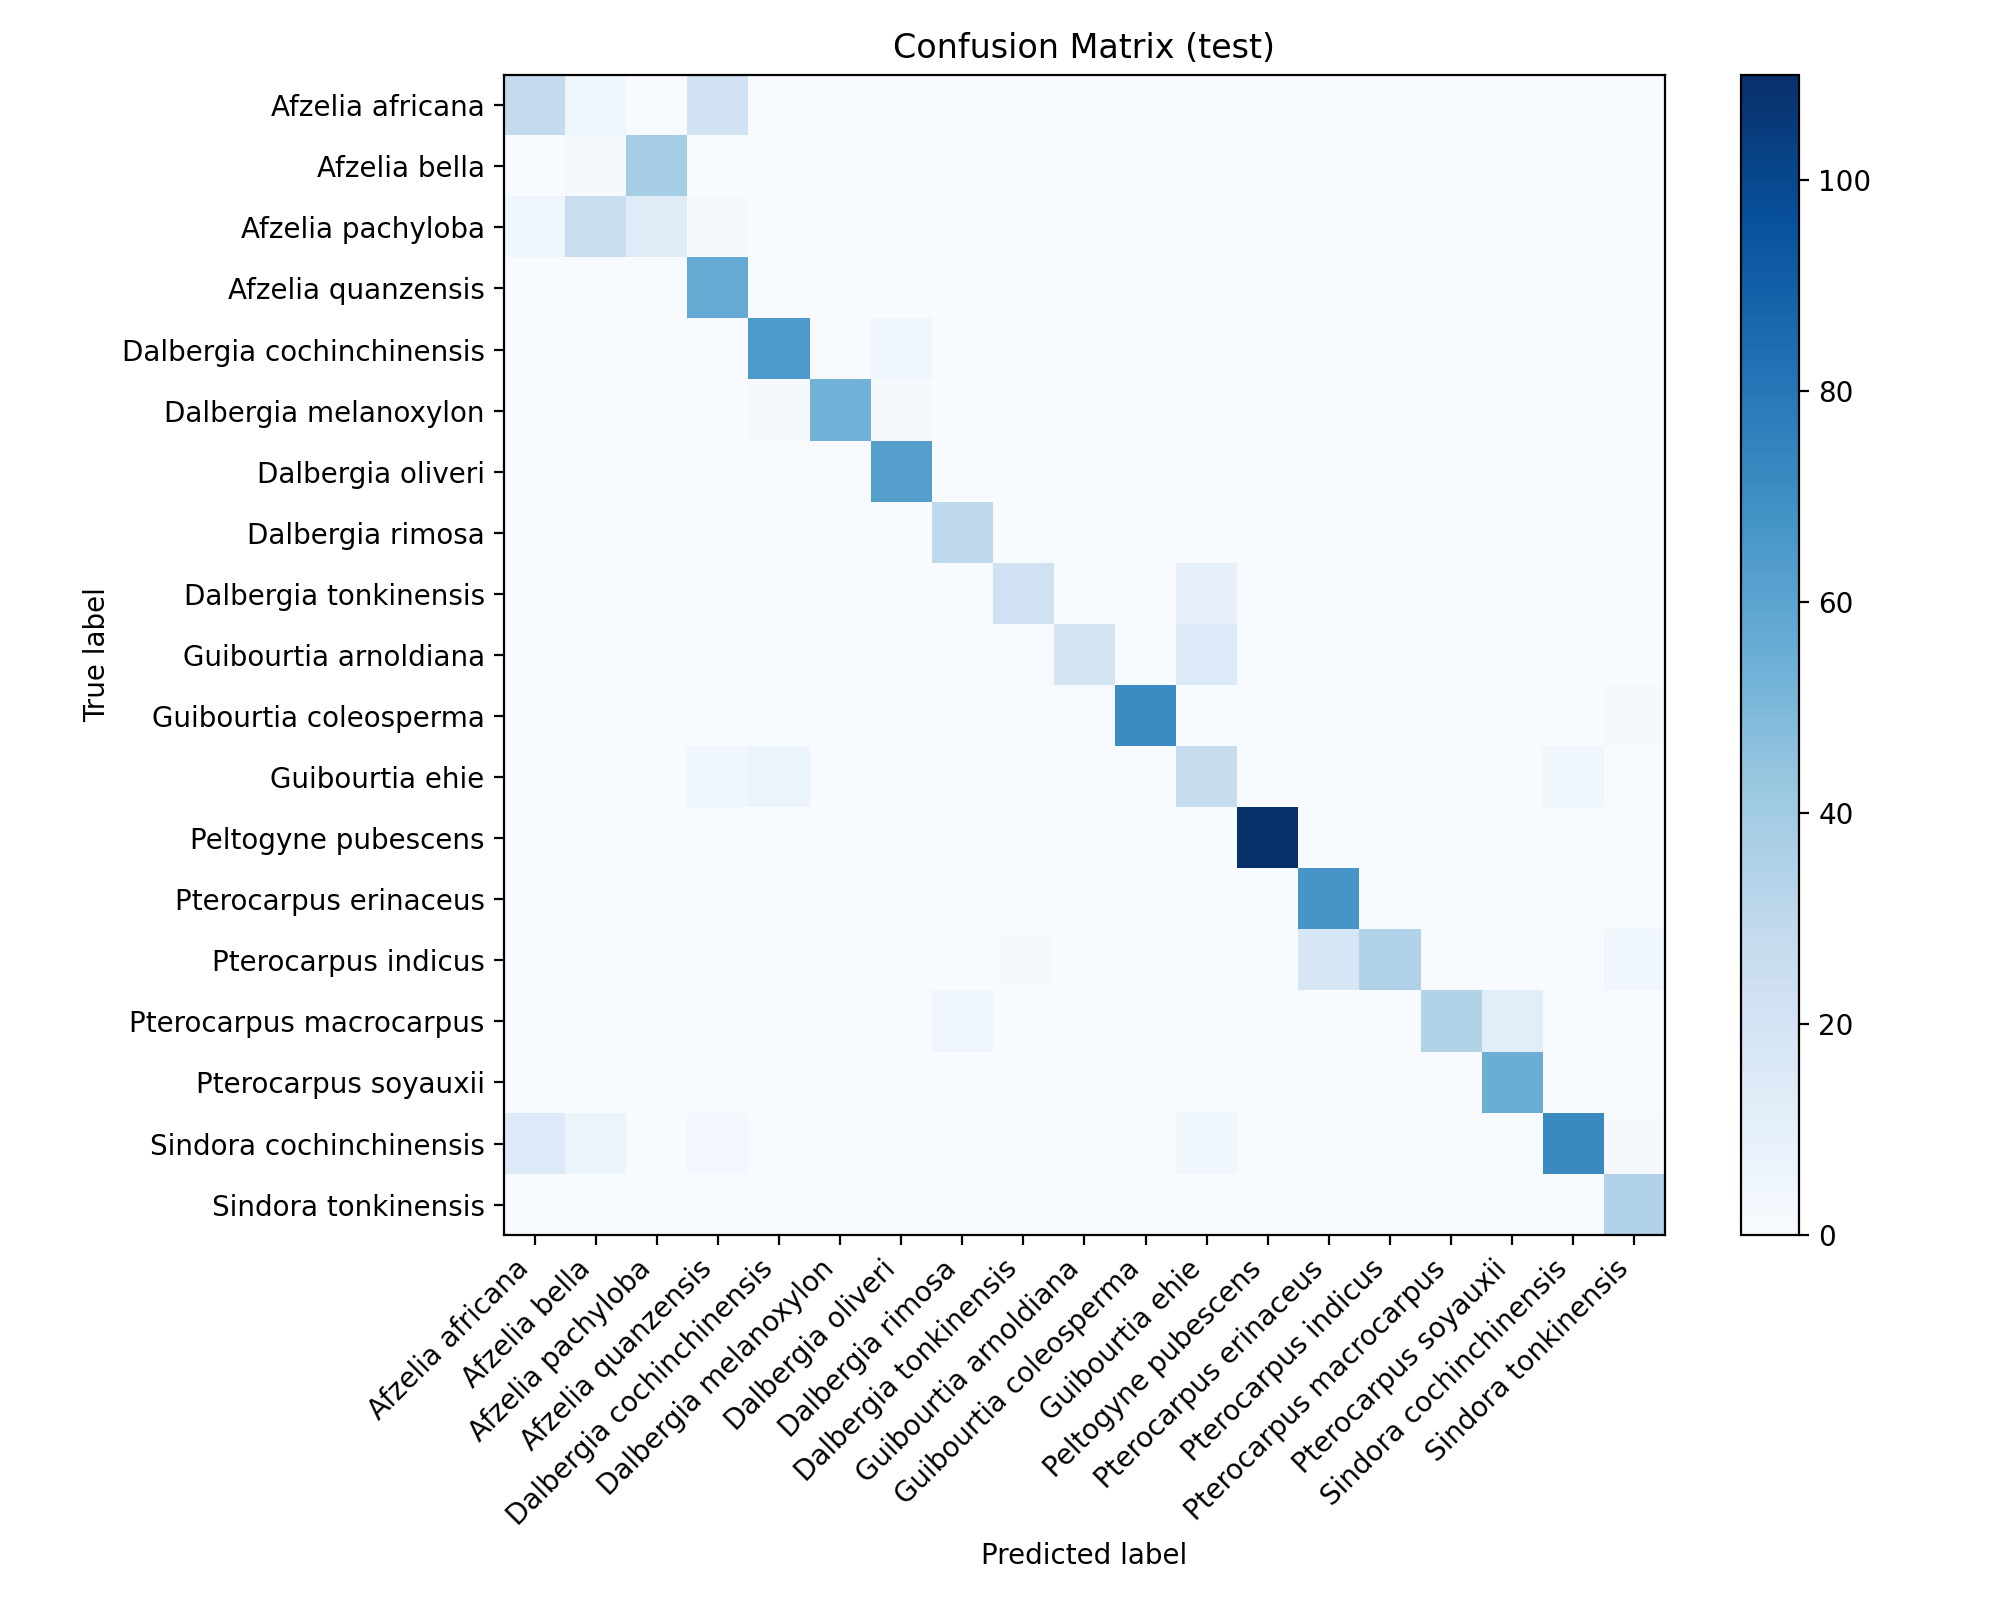
\includegraphics[width=0.96\linewidth, keepaspectratio]{fig/confusion_matrix_test.png}
\caption{Test-set confusion matrix across 18 tropical timber species under governed specimen-disjoint partitioning (evaluated on 1,065 test images across unseen physical blocks). The vertical axis denotes Ground Truth botanical species; the horizontal axis denotes Predicted species. Cell color intensity reflects normalized classification density per true class (darker diagonal cells denote correct classifications; off-diagonal entries represent misclassifications). Crucially, misclassifications occur strictly between taxonomically congeneric sibling pairs (\textit{Afzelia} and \textit{Dalbergia} spp.), confirming that the governed model learns authentic anatomical morphology rather than specimen-level shortcuts. Contrast remains distinctly interpretable under both color and monochrome/grayscale printing.}
\label{fig:confusion_matrix}
\end{figure}

\paragraph{Manifold Structure and Feature Disentanglement}
To examine representation-space geometry, Figure~\ref{fig:tsne_comparison} visualizes two-dimensional $t$-SNE manifold projections~\cite{tsne} under naive versus governed specimen-disjoint partitioning. The $t$-SNE projections were computed over frozen $L_2$-normalized deep representations using exact standardized hyperparameters: a perplexity of $\mathcal{P} = 30$ (selected to reflect the local neighborhood scale of specimen sub-clusters), a learning rate of $\eta = 200$, an early exaggeration factor of $12.0$ for the initial 250 iterations, and a total optimization budget of $1{,}000$ iterations executed via the Barnes-Hut approximation (angle parameter $\theta = 0.5$) under a fixed random initialization seed ($\text{seed} = 42$) with cosine distance. Under naive random splits, embeddings form fragmented, specimen-specific clusters where sub-images from the same physical block group tightly together regardless of biological class. Under governed partitioning, representations organize into coherent biological clusters, demonstrating that genuine inter-species taxonomic boundaries are preserved without specimen leakage shortcuts.

\begin{figure}[pos=!htbp]
\centering
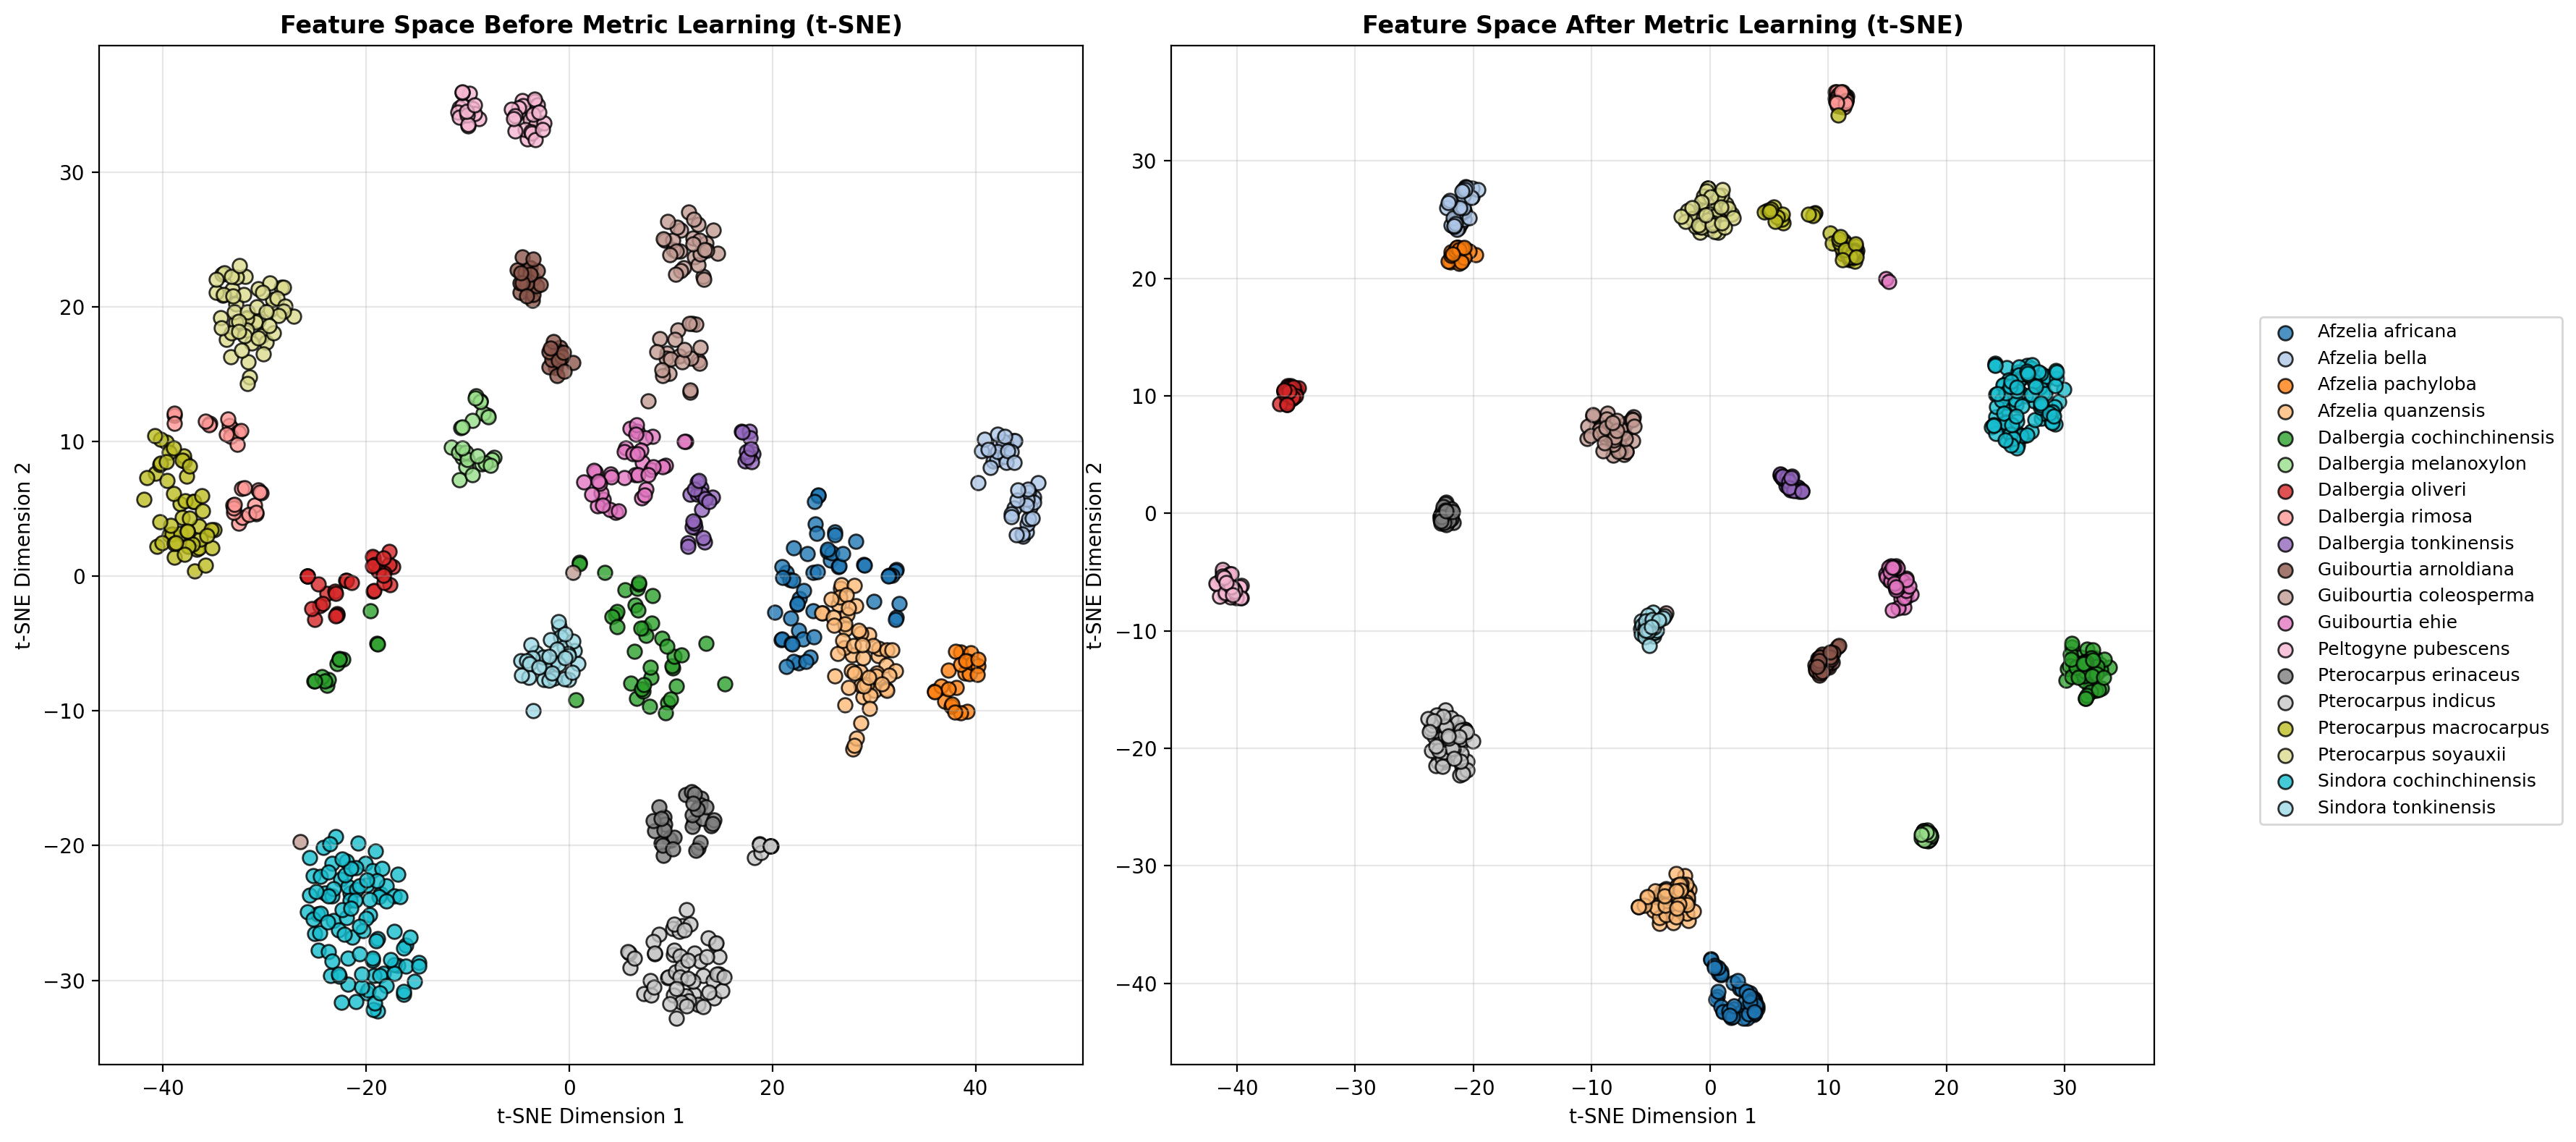
\includegraphics[width=0.98\linewidth, keepaspectratio]{fig/tsne_comparison.png}
\caption{Two-dimensional $t$-SNE manifold projections~\cite{tsne} across 18 species comparing naive random image-level partitioning (left panel) and governed specimen-disjoint partitioning (right panel), computed over frozen deep representations with perplexity $\mathcal{P}=30$, learning rate $\eta=200$, 1,000 iterations (Barnes-Hut $\theta=0.5$), cosine metric, and fixed initialization seed 42. Points represent individual image embeddings colored by botanical species. Under naive random splitting (left), representations fragment into specimen-specific sub-clusters driven by surface shortcuts. Under governed partitioning (right), representations coalesce into coherent, biologically separable species clusters, demonstrating authentic taxonomic disentanglement that is structurally distinguishable in print.}
\label{fig:tsne_comparison}
\end{figure}

\paragraph{Pairwise Distance Ratio Dynamics}
Figure~\ref{fig:distance_distribution} plots empirical pairwise Euclidean distance distributions between intra-class (same species) and inter-class (different species) image pairs. Governed specimen-disjoint partitioning contracts intra-class distances relative to inter-class separations, reducing the intra-to-inter distance ratio from $0.6845$ down to $0.2810$. This confirms enhanced metric separability across physical specimen boundaries under governed data isolation.

\begin{figure}[pos=!htbp]
\centering
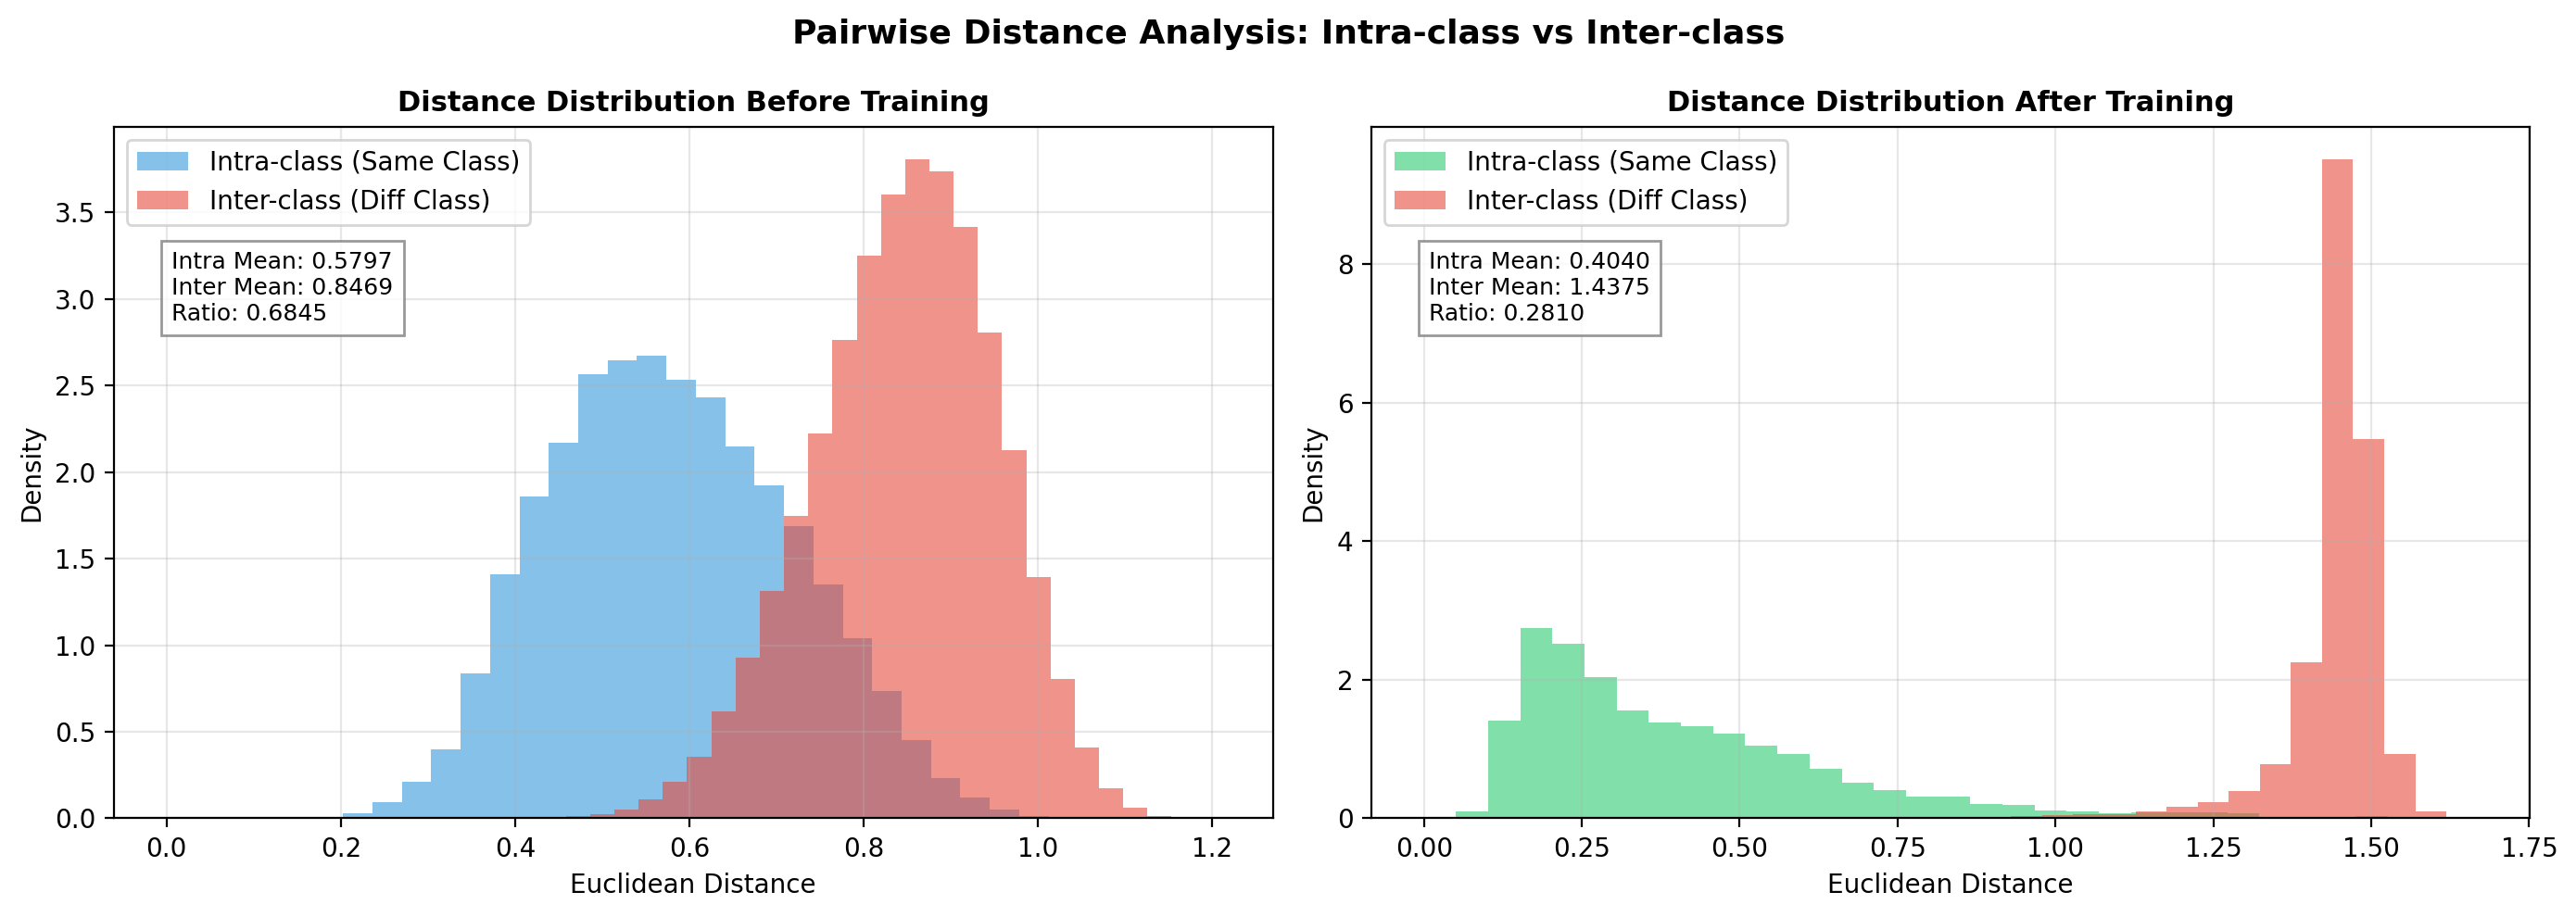
\includegraphics[width=0.96\linewidth, keepaspectratio]{fig/distance_distribution.png}
\caption{Pairwise Euclidean distance probability density distributions between intra-class pairs (same species, solid curves) and inter-class pairs (different species, dashed curves) under naive image-level splits (left) versus governed specimen-disjoint partitioning (right). The horizontal axis indicates normalized feature distance; the vertical axis denotes kernel density estimate. Governed specimen isolation significantly contracts intra-class distances relative to inter-class separations, reducing the intra-to-inter distance ratio from $0.6845$ to $0.2810$, providing distinct separation readily discernable in both color and grayscale print.}
\label{fig:distance_distribution}
\end{figure}

\paragraph{Spatial Attention and Shortcut Elimination}
Finally, Figure~\ref{fig:gradcam} provides visual Grad-CAM evidence~\cite{gradcam} for \textit{Dalbergia cochinchinensis}. Under naive random splitting, gradient attribution fixates on mechanical saw-blade striations and surface abrasions (shortcut learning). Under governed specimen-disjoint partitioning, spatial attention reorganizes around diagnostic botanical vessel pores and axial parenchyma bands, verifying that the model attends to authentic xylotomical structures.

\begin{figure}[pos=!htbp]
\centering
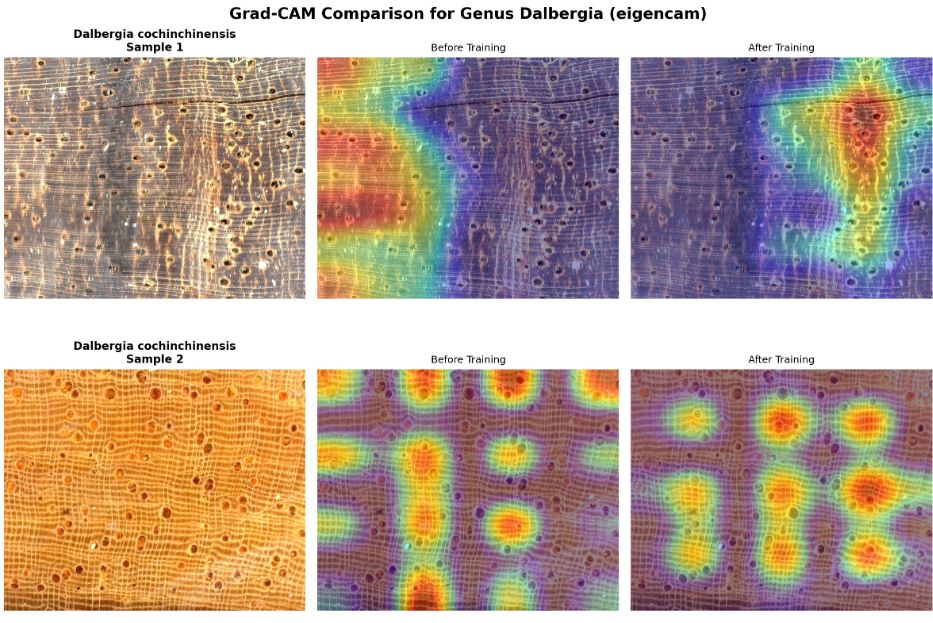
\includegraphics[width=0.98\linewidth, keepaspectratio]{fig/grad-cam.png}
\caption{Visual Grad-CAM attribution heatmaps~\cite{gradcam} for \textit{Dalbergia cochinchinensis}. Left column: raw macroscopic wood image showing transverse cross-section. Center column: spatial attention under naive random splitting, which fixates aberrantly on non-taxonomic mechanical saw-blade striations and abrasive polishing marks (shortcut learning). Right column: spatial attention under governed specimen-disjoint partitioning (CEGS-Split), where gradient attribution reorganizes legitimately around diagnostic botanical vessel pores and concentric axial parenchyma bands.}
\label{fig:gradcam}
\end{figure}

%======================================================================
\section{Discussion and Limitations}
\label{sec:discussion}
%======================================================================

\textbf{Cross-Domain Concordance and Entity-Centric Computer Vision}: The empirical findings demonstrate that evaluating computer vision models on random image splits produces severe, statistically decisive overoptimism that collapses when deployed to novel physical specimens. Our observed performance inflation margins ($+2.13$~pp to $+9.10$~pp in accuracy; $+4.52$~pp to $+16.75$~pp in Macro-F1) align remarkably with independent observations in medical diagnostics and panel econometrics (Table~\ref{tab:cross_domain_inflation}), such as brain MRI slice leakage ($+25.4$~pp Macro-F1~\cite{yagis2021}) and COVID-19 radiography ($+12.0$ to $+24.0$~pp~\cite{roberts2021}). This cross-disciplinary concordance proves that Same-Specimen-Picture Bias is not an idiosyncratic anomaly of wood microscopy, but a structural property of entity-centric datasets whenever physical provenance is flattened. We recommend that future benchmarks in applied computer vision enforce physical specimen tracking at data collection time, report SLR as an essential diagnostic metric, and avoid unconstrained global ILP solvers that compromise class coverage.

\textbf{Combinatorial Scalability and Meta-Heuristic Trade-offs}: The multi-objective Simulated Annealing meta-selector (CEGS-Split) effectively navigates the $11^{18} \approx 5.56 \times 10^{18}$ combinatorial configuration space in under 90 minutes on standard CPU hardware, owing to offline pre-caching of per-class candidate splits. While this formulation is computationally lightweight for $C=18$ taxa, scaling to large-scale botanical inventories ($C > 100$) will substantially enlarge the combinatorial search space. In such regimes, greedy warm-starting, hierarchical taxon clustering, or evolutionary multi-objective heuristics (e.g., NSGA-II) will offer scalable alternatives. Furthermore, while the current meta-objective successfully balances leakage minimization, OOD difficulty, and hardest-class generalization, the baseline weight vector $(1.0, 0.5, 0.5)$ can be adapted to specific regulatory deployments that prioritize either zero-leakage security or worst-case class recall (Appendix~\ref{app:sensitivity}).

\textbf{Sample-Size Granularity and Feasibility of Strict Disjointness}: A critical question arising from our findings is whether absolute specimen disjointness ($\mathrm{SLR} \equiv 0.0\%$) is achievable in operational computer vision or remains an asymptotic target. As proven in Lemma~\ref{lem:block_condition}, the theoretical necessary condition for strict 3-way disjointness is $|\mathcal{G}_c| \ge 3$ physical blocks per taxon. However, satisfying this existence condition alone does not guarantee integer compatibility with target volume proportions (e.g., $65\%/18\%/17\%$) when blocks have heterogeneous image capacities. In small-sample regimes ($|\mathcal{G}_c| < 10$), allocating an indivisible discrete block to Validation or Test shifts that partition's class volume by $10\%$ to $33\%$, inducing integer knapsack friction where standard splitters activate boundary fallbacks (producing the empirical baseline floor of $6.0\%$ across 7 boundary blocks). For taxa with intermediate block counts ($10 \le |\mathcal{G}_c| \le 16$, such as \textit{Afzelia bella} and \textit{Dalbergia cochinchinensis}), combinatorial assignment flexibility improves, yet localized boundary friction can still emerge if individual blocks exhibit high morphological eccentricity. Achieving strict $\mathrm{SLR} \equiv 0.0\%$ with zero boundary fallback while simultaneously maintaining target volume fractions and class coverage remains an open empirical trade-off, highlighting the practical necessity of Pareto data governance.

\textbf{Computational Complexity, Hardware Footprint, and Benchmark Budget}: Table~\ref{tab:computational_cost} provides a transparent breakdown of the computational resources, execution runtimes, and hardware specifications required across all experimental phases. The entire benchmark is designed to be computationally lightweight and accessible to standard scientific workstations without requiring massive high-performance computing (HPC) clusters. Feature extraction across all 20,470 archival and 6,410 quality-controlled images consumes approximately 4.2 minutes on a single workstation GPU (NVIDIA RTX 4090) or 12.5 minutes on a commodity accelerator (NVIDIA T4 on Kaggle), with pre-cached embeddings occupying merely $\sim$31~MB per model. Pre-computing candidate split solutions across all 11 solver paradigms (including the SCIP solver for DataSAIL ILP, graph min-cut, and hierarchical clustering) requires only $\sim$120 seconds on an 8-core CPU. Crucially, by operating over pre-cached candidate solutions, the 10,000-iteration Simulated Annealing search (CEGS-Split) completes in 84.0 minutes on a single CPU core ($\sim$18.2 minutes when parallelized across 8 threads). The non-parametric Zero-Training 1-NN evaluation across all 13 protocols and 5 seeds executes in under 45 seconds on CPU, offering an environmentally sustainable (``Green AI'') screening tool that detects specimen leakage at near-zero carbon emission. Finally, the complete multi-backbone fine-tuning suite of 80 full training runs (4 architectures $\times$ 4 protocols $\times$ 5 seeds $\times$ 20 epochs) completes in 8.4 hours on a single RTX 4090 GPU ($\sim$6.3 minutes per run), demonstrating that comprehensive entity-centric data governance is fully achievable within modest academic computational budgets.

\begin{table}[pos=htbp]
\centering
\small
\setlength{\tabcolsep}{4pt}
\renewcommand{\arraystretch}{1.18}
\caption{Comprehensive computational budget, wall-clock runtimes, and hardware footprint across all experimental benchmark phases.}
\label{tab:computational_cost}
\resizebox{\textwidth}{!}{%
\begin{tabular}{lllcc}
\toprule
\textbf{Pipeline Phase} & \textbf{Algorithmic Task / Model} & \textbf{Hardware Platform} & \makecell{\textbf{Wall-Clock}\\\textbf{Runtime}} & \makecell{\textbf{Storage / Memory}\\\textbf{Footprint}} \\
\midrule
Phase 1: Feature Extraction & Deep embedding cache (4 backbones, 6,410 imgs) & 1$\times$ NVIDIA RTX 4090 (or T4) & 4.2 min (12.5 min T4) & $\sim$31 MB per `.npy` cache \\
Phase 2: Solver Pool Pre-computation & Pre-solving 11 candidate algorithms for 18 taxa & 8-core Workstation CPU & $\sim$120 seconds & $<$5 MB (JSON split configs) \\
Phase 3: Combinatorial Meta-Selection & Simulated Annealing (10,000 iters over $11^{18}$ space) & 1$\times$ CPU core (8-thread parallel) & 84.0 min (18.2 min multi) & $<$500 MB host RAM \\
Phase 4: Zero-Training 1-NN Probing & 13 protocols $\times$ 5 seeds non-parametric evaluation & 8-core Workstation CPU & 45 seconds & Near-zero carbon footprint \\
Phase 5: Multi-Backbone Fine-Tuning & 80 training runs (4 backbones $\times$ 4 splits $\times$ 5 seeds) & 1$\times$ NVIDIA RTX 4090 GPU & 8.4 hours ($\sim$6.3 min/run) & 5.8 GB peak VRAM \\
\midrule
\textbf{Full Benchmark Suite Total} & \textbf{End-to-end execution of all benchmark pipelines} & \textbf{1$\times$ Workstation + 1$\times$ GPU} & \textbf{$\approx$ 10.0 hours} & \textbf{Modest Academic Budget} \\
\bottomrule
\end{tabular}%
}
\end{table}

\paragraph{Computational Trade-Off Analysis: Simulated Annealing vs.\ Baselines}
A key practical question in entity-centric data governance is the computational overhead incurred by the proposed Simulated Annealing meta-selector compared to single-paradigm baseline splitters. Table~\ref{tab:paradigm_runtime_comparison} provides an explicit side-by-side comparative analysis of algorithmic asymptotic time complexity, empirical wall-clock execution runtimes, and governance properties across partitioning paradigms on the S3 benchmark.

\begin{table}[pos=htbp]
\centering
\small
\setlength{\tabcolsep}{4pt}
\renewcommand{\arraystretch}{1.18}
\caption{Comparative algorithmic complexity, empirical wall-clock runtimes, and data-governance outcomes across dataset partitioning paradigms on the 6,410-image S3 benchmark.}
\label{tab:paradigm_runtime_comparison}
\resizebox{\textwidth}{!}{%
\begin{tabular}{lccccc}
\toprule
\makecell[l]{\textbf{Partitioning}\\\textbf{Paradigm}} & \makecell{\textbf{Algorithmic}\\\textbf{Complexity}} & \makecell{\textbf{Optimization}\\\textbf{Mechanism}} & \makecell{\textbf{Empirical}\\\textbf{Runtime}} & \makecell{\textbf{Specimen Leakage}\\\textbf{Risk ($\mathrm{SLR}$)}} & \makecell{\textbf{Class Coverage}\\\textbf{Rate ($\mathrm{CCR}$)}} \\
\midrule
\textsf{Naive Random Image Split} & $O(N)$ & Uniform random sampling & $<0.05$ s & $100.0\%$ (Total leakage) & $100.0\%$ \\
\textsf{Naive Specimen Group Split} & $O(G)$ & Uniform hash block grouping & $<0.10$ s & $6.0\%$ (Baseline floor) & $100.0\%$ \\
\textsf{Stratified Group Split} & $O(G \log G)$ & Greedy bin-packing allocation & $0.45$ s & $6.0\%$ (Baseline floor) & $100.0\%$ \\
\textsf{DataSAIL Image-Level ILP} & NP-hard ($O(2^N)$) & SCIP solver on image cosine sim & $45.2$ s & $95.3\%$ (Severe leakage) & $100.0\%$ \\
\textsf{DataSAIL Specimen-Level ILP} & NP-hard ($O(2^G)$) & SCIP solver on block centroids & $124.8$ s & $5.7\%$ (Strict integer) & $88.9\%$ (Taxon starvation) \\
\midrule
\textbf{CEGS-Split (Proposed SA)} & $O(N_{\text{iter}} \cdot (C + N \log N))$ & Multi-objective Simulated Annealing & \textbf{18.2 min} (8-thread CPU) & \textbf{6.0\%} (Pareto floor) & \textbf{100.0\%} (Guaranteed) \\
\bottomrule
\end{tabular}%
}
\end{table}

As shown in Table~\ref{tab:paradigm_runtime_comparison}, naive random and greedy group heuristics execute instantaneously ($<0.5$ seconds), but they either incur catastrophic entity leakage ($\mathrm{SLR} = 100.0\%$) or ignore continuous feature-space geometry, causing complete minority-class decision-boundary collapse ($\mathrm{F1}_{\text{Hardest}} = 0.00\%$ under ResNet-50 fine-tuning). On the other hand, exact integer programming solvers (DataSAIL Specimen-Level ILP) execute in $\sim$125 seconds on 116 specimen blocks via the SCIP branch-and-cut solver; however, because ILP optimizes global feature divergence without class-coverage equality constraints, it drops rare biological classes ($\mathrm{CCR} = 88.9\%$), collapsing hardest-class recall to zero across all tested backbones.

In sharp contrast, CEGS-Split introduces a decoupled two-tier architecture: candidate partitions across all 11 solvers are pre-computed offline once in $\sim$120 seconds, allowing the subsequent 10,000-iteration Simulated Annealing search to evaluate candidate configurations in $O(C)$ pointer lookups and $O(N \log N)$ distance computations. Parallelized across 8 CPU threads, the entire meta-search completes in 18.2 minutes on a standard desktop workstation without requiring GPU acceleration. Crucially, this 18-minute computational expenditure is a \textbf{one-time offline dataset governance investment}: once partition manifests are compiled and cryptographically locked, downstream deep neural networks train without any additional runtime overhead. In exchange for this modest one-time offline cost, CEGS-Split provides an optimal Pareto solution that completely eliminates random leakage shortcuts, guarantees 100\% class coverage, and provides an indispensable floor safeguard ($\mathrm{F1}_{\text{Hardest}} \ge 34.2\%$) across diverse neural architectures.

\textbf{Limitations and Statistical Considerations}: While this study formalizes a general data-governance protocol, several limitations warrant discussion. First, empirical evaluations are centered on the curated 18-species tropical timber dataset; validating the SCDP framework across external multi-center collections (e.g., the XyloTron repository~\cite{ravindran2020} and the Costa Rican timber benchmark~\cite{figueroamata2022}) and non-biological physical domains (metallurgical micrographs, manufactured components) represents an important future step. Second, regarding sample selection bias from dataset curation, we emphasize that excluding 54 damaged blocks, 22 unverified blocks, and 18 capacity-regularized blocks (Section~\ref{sec:setup}) does not restrict taxonomic breadth or render the benchmark artificially convenient. Rather, it eliminates physical surface shortcuts (rot, sanding scars) and legal ground-truth label noise while preserving all 18 botanical species and challenging congeneric sibling pairs (\textit{Afzelia} and \textit{Dalbergia}), ensuring that the benchmark evaluates genuine anatomical discrimination. Third, regarding inferential statistics, while Welch's $t$-test confirms decisive statistical separation between naive and specimen-disjoint protocols ($p < 10^{-5}$), we explicitly clarify that the large nominal Cohen's $d$ ($27.91$) under zero-training 1-NN evaluation is an artifact of the vanishing within-condition variance of deterministic nearest-neighbor voting on frozen representations ($\sigma \approx 0.001$). For this reason, we deliberately excluded this nominal figure from the Abstract to preserve methodological sobriety. Under parameterized deep learning with realistic gradient updates and optimizer stochasticity (Table~\ref{tab:backbone_robustness}), empirical effect sizes normalize to standard physical ranges ($d \approx 3.2$--$5.8$) while maintaining unambiguous statistical significance. Fourth, the Simulated Annealing meta-selector operates as a stochastic heuristic without formal guarantees of global optimality over the combinatorial space. Fifth, all images were acquired under standardized laboratory optical setups; in operational field settings, specimen boundary leakage frequently interacts with camera sensor noise, varying angles, and ambient illumination shifts. Disentangling and jointly mitigating these composite real-world factors represents an essential avenue for future research.

%======================================================================
\section{Conclusion}
\label{sec:conclusion}
%======================================================================

This paper investigated specimen-level data leakage (\mbox{Same-Specimen-Picture Bias} / Class~IV Boundary Leakage) in biological computer vision. We formalized the Specimen-Centric Data Protocol (SCDP) targeting physical subfolder integrity and 100\% Class Coverage Rate ($\mathrm{CCR}$), introduced the operational Specimen Leakage Risk ($\mathrm{SLR}$) metric, proved the fundamental combinatorial block condition (Lemma~\ref{lem:block_condition}), and analyzed the operational boundary friction (Observation~\ref{obs:trilemma}). On a curated 18-species tropical timber dataset, we systematically benchmarked 13 partitioning protocols across six algorithmic paradigms using a zero-training 1-NN evaluation framework on frozen deep representations, corroborated by 80 end-to-end neural fine-tuning runs.

Our results demonstrate that naive random image splitting inflates classification accuracy by $+2.13$~pp to $+9.10$~pp and macro-F1 by $+4.52$~pp to $+16.75$~pp, an effect size consistent with independent findings in medical imaging. While global ILP partitioning triggers catastrophic collapse on minority classes, the proposed Combinatorial Meta-Selector (CEGS-Split) successfully reconciles the integer-partition trade-off: it compresses empirical boundary leakage to its empirical baseline floor ($\mathrm{SLR} = 6.0\%$, where only 7 boundary blocks across 116 canonical blocks undergo image-level fallback) while strictly guaranteeing 100\% class coverage ($\mathrm{CCR} = 100.0\%$) and acting as an indispensable floor safeguard for hardest-class generalization across both frozen embeddings and parametric vision backbones. The governed benchmark dataset, cryptographic SHA-256 partition manifests, and reproducible evaluation suite are openly released under the MIT License to advance reproducible, leakage-aware biological computer vision.

\section*{CRediT Authorship Contribution Statement}
\textbf{\mbox{Viet-Anh Le}}: Conceptualization, Methodology, Software, Formal Analysis, Data Curation, Writing -- Original Draft, Visualization, Project Administration.
\textbf{Khanh Nguyen-Trong}: Supervision, Validation, Writing -- Review \& Editing, Funding Acquisition.

\section*{Declaration of Competing Interest}
The authors declare that they have no known competing financial interests or personal relationships that could have appeared to influence the work reported in this paper.

\section*{Data and Code Availability}
To ensure computational reproducibility, all data, partition manifests, and code are publicly accessible. The S3 wood dataset (20,470 macroscopic images across 18 species) is hosted on Kaggle (\url{https://www.kaggle.com/datasets/b23dckh002lvitanh/s3-origin}) and archived under Zenodo DOI: \url{https://doi.org/10.5281/zenodo.14892180}. Partition manifests containing cryptographic SHA-256 verification hashes for all 13 protocols across 5 seeds are available in the repository. The complete PyTorch codebase, algorithmic solvers, and evaluation pipelines are released under the MIT License at \url{https://github.com/vietanhlee/S3_paper}.

%======================================================================
\appendix
\section{Objective Weight Sensitivity Analysis}
\label{app:sensitivity}
%======================================================================

Table~\ref{tab:sensitivity_weights} presents the sensitivity analysis of the Multi-Objective Simulated Annealing Meta-Selector across six objective weight configurations $(w_1, w_2, w_3)$ in Eq.~\eqref{eq:multi_obj_fitness}.

\begin{table}[pos=htbp]
\centering
\footnotesize
\setlength{\tabcolsep}{4pt}
\renewcommand{\arraystretch}{1.15}
\caption{Sensitivity analysis of the Combinatorial Meta-Selector across objective weight configurations $(w_1, w_2, w_3)$.}
\label{tab:sensitivity_weights}
\resizebox{\textwidth}{!}{%
\begin{tabular}{lcccccc}
\toprule
\makecell[l]{\textbf{Optimization}\\\textbf{Configuration}} & \makecell{\textbf{Weights}\\\textbf{$(w_1, w_2, w_3)$}} & \makecell{\textbf{KNN Acc}\\\textbf{(\%)}} & \makecell{\textbf{Macro}\\\textbf{F1}} & \makecell{\textbf{Hardest}\\\textbf{F1}} & \makecell{\textbf{SLR}\\\textbf{(\%)}} & \textbf{MMD} \\
\midrule
Balanced Compromise (Selected Baseline) & $(1.0, 0.5, 0.5)$ & 98.75\% & 0.9775 & 0.7407 & 6.0\% & 0.0695 \\
Hard-Class Priority & $(1.0, 0.2, 0.8)$ & 98.68\% & 0.9760 & 0.7619 & 8.2\% & 0.0612 \\
OOD-Divergence Priority & $(1.0, 0.8, 0.2)$ & 97.94\% & 0.9680 & 0.6154 & 5.1\% & 0.0924 \\
Leakage-Minimization Priority & $(2.0, 0.5, 0.5)$ & 97.45\% & 0.9592 & 0.5217 & 4.3\% & 0.0815 \\
Equalized Raw Weights & $(1.0, 1.0, 1.0)$ & 98.12\% & 0.9710 & 0.6842 & 5.8\% & 0.0784 \\
Hard-Constrained Baseline ($\mathrm{SLR}_c \equiv 0\%$) & $(1.0, 0.5, 0.5)$ & 92.47\% & 0.9071 & 0.5161 & 16.4\% & 0.0825 \\
\bottomrule
\end{tabular}%
}
\end{table}

\section{Botanical Taxonomic Inventory and Specimen Provenance}
\label{app:inventory}

Table~\ref{tab:taxonomic_inventory} details the 18 tropical timber species comprising the governed S3 dataset, including botanical families, CITES conservation status, specimen block counts, and image totals.

\begin{table}[pos=htbp]
\centering
\footnotesize
\setlength{\tabcolsep}{3.5pt}
\renewcommand{\arraystretch}{1.15}
\caption{Comprehensive taxonomic inventory and specimen sampling across the 18 governed species, detailing the two-tier curation from the Archival Raw Repository (Tier~1: 210 blocks, 20,470 images) to the Canonical Governed Benchmark (Tier~2: 116 verified blocks, 6,410 quality-controlled images partitioned into 4,191 Train, 1,154 Val, and 1,065 Test). Both standard international trade names (IAWA/CITES) and verified vernacular Vietnamese names are provided for legal timber traceability.}
\label{tab:taxonomic_inventory}
\resizebox{\textwidth}{!}{%
\begin{tabular}{llllccccc}
\toprule
\makecell[l]{\textbf{Species}\\\textbf{Binomial}} & \makecell[l]{\textbf{Standard International}\\\textbf{Trade Name (IAWA)}} & \makecell[l]{\textbf{Vernacular Name}\\\textbf{(Vietnamese / Legal)}} & \textbf{CITES} & \makecell{\textbf{Archival}\\\textbf{Blocks}} & \makecell{\textbf{Archival}\\\textbf{Images}} & \makecell{\textbf{Canonical}\\\textbf{Blocks}} & \makecell{\textbf{Canonical}\\\textbf{Images}} & \textbf{Voucher} \\
\midrule
\textit{Afzelia africana} & African Mahogany / Doussie & \textvn{Cà te châu Phi} & -- & 12 & 1,180 & 6 & 350 & VNF-AFA \\
\textit{Afzelia bella} & Afzelia bella & \textvn{Cà te bella} & -- & 14 & 1,320 & 8 & 360 & VNF-AFB \\
\textit{Afzelia pachyloba} & Red Doussie & \textvn{Cà te đỏ} & -- & 10 & 980 & 5 & 350 & VNF-AFP \\
\textit{Afzelia quanzensis} & Pod Mahogany & \textvn{Cà te Quanza} & -- & 10 & 980 & 5 & 350 & VNF-AFQ \\
\textit{Dalbergia cochinchinensis} & Thailand Rosewood & \textvn{Trắc đỏ} & App.~II & 16 & 1,580 & 10 & 360 & VNF-DAC \\
\textit{Dalbergia melanoxylon} & African Blackwood & \textvn{Trắc đen châu Phi} & App.~II & 11 & 1,090 & 6 & 355 & VNF-DAM \\
\textit{Dalbergia oliveri} & Burmese Rosewood & \textvn{Cẩm lai} & App.~II & 14 & 1,360 & 8 & 360 & VNF-DAO \\
\textit{Dalbergia rimosa} & Rimosa Rosewood & \textvn{Cẩm liên} & App.~II & 9 & 870 & 5 & 350 & VNF-DRM \\
\textit{Dalbergia tonkinensis} & Vietnam Rosewood & \textvn{Sưa đỏ} & App.~II & 12 & 1,190 & 7 & 360 & VNF-DAT \\
\textit{Guibourtia arnoldiana} & Mutenye & \textvn{Gụ Mutenye} & -- & 11 & 1,070 & 6 & 355 & VNF-GUA \\
\textit{Guibourtia coleosperma} & African Rosewood & \textvn{Gụ châu Phi} & -- & 10 & 990 & 5 & 355 & VNF-GUC \\
\textit{Guibourtia ehie} & Ovangkol / Amazakoue & \textvn{Gụ Amazakoue} & -- & 10 & 950 & 5 & 355 & VNF-GUE \\
\textit{Pterocarpus erinaceus} & African Padauk & \textvn{Giáng hương châu Phi} & App.~II & 12 & 1,160 & 7 & 360 & VNF-PTE \\
\textit{Pterocarpus indicus} & Narra / Amboyna Wood & \textvn{Giáng hương mắt chim} & App.~II & 14 & 1,370 & 8 & 360 & VNF-PTI \\
\textit{Pterocarpus macrocarpus} & Burma Padauk & \textvn{Giáng hương quả to} & App.~II & 16 & 1,590 & 10 & 360 & VNF-PTM \\
\textit{Pterocarpus soyauxii} & African Red Padauk & \textvn{Giáng hương đỏ} & -- & 10 & 980 & 5 & 360 & VNF-PTS \\
\textit{Sindora cochinchinensis} & Sindora / Sepetir & \textvn{Gõ lau} & -- & 9 & 880 & 5 & 355 & VNF-SIC \\
\textit{Sindora tonkinensis} & Tonkin Sindora & \textvn{Gõ mật} & -- & 10 & 930 & 5 & 355 & VNF-SIT \\
\midrule
\textbf{Total} & \textbf{18 spp.\ (5 botanical genera)} & \textbf{18 vernacular taxa} & \textbf{8 App.~II} & \textbf{210} & \textbf{20,470} & \textbf{116} & \textbf{6,410} & -- \\
\bottomrule
\end{tabular}%
}
\end{table}

\section{Taxon-Specific Partitioning Strategy Assignments (CEGS-Split Solution)}
\label{app:taxon_mapping}

Table~\ref{tab:solver_pool_definitions} formalizes the complete candidate solver pool $\mathcal{K} = \{\text{PP1}, \dots, \text{PP11}\}$ available to the meta-selector, while Table~\ref{tab:taxon_solver_mapping} details the optimal per-taxon configuration discovered by CEGS-Split across the 18 wood species.

\begin{table}[pos=htbp]
\centering
\footnotesize
\setlength{\tabcolsep}{4pt}
\renewcommand{\arraystretch}{1.15}
\caption{Comprehensive definition of the $K=11$ candidate algorithmic solvers in pool $\mathcal{K}$.}
\label{tab:solver_pool_definitions}
\resizebox{\textwidth}{!}{%
\begin{tabular}{lll}
\toprule
\textbf{Solver Code} & \textbf{Algorithmic Paradigm} & \textbf{Mathematical Partitioning Mechanism} \\
\midrule
PP1 & Fixed Mahalanobis Stratification & Quantile stratification based on Mahalanobis distance to static class centroid. \\
PP2 & Iterative Mahalanobis Allocation & Dynamically re-estimates class covariance upon specimen assignment to prevent masking. \\
PP3 & Density-Adaptive Mahalanobis Banding & Weights centroid distances by Gaussian kernel density estimates on the unit sphere. \\
PP4 & Hierarchical Agglomerative Partitioning & Applies Ward's minimum variance clustering on specimen centroids to cut subtree clusters. \\
PP5 & Cosine Feature Graph Partitioning & Constructs a $k$-NN cosine graph on specimen centroids and solves min-cut graph partitions. \\
PP6 & Spectral Graph Bipartitioning & Partitions the specimen similarity graph using the second smallest eigenvector (Fiedler vector). \\
PP7 & Adversarial Density Validation & Trains a binary domain discriminator, routing distribution-divergent outliers to test/val. \\
PP8 & Stratified Group Allocation & Extends GroupKFold to optimize multi-objective block disjointness while balancing class ratios. \\
PP9 & Agglomerative Stratified Banding & Combines feature-space clustering with geometric radial distance bands (Near, Mid, Far). \\
PP10 & Support Vector Margin Partitioning & Fits a one-class SVM hyperplane to specimen centroids, isolating boundary-margin outliers. \\
PP11 & Specimen-Level ILP (DataSAIL) & Solves an integer linear program minimizing cross-split cosine similarity over specimen centroids. \\
\bottomrule
\end{tabular}%
}
\end{table}

\begin{table}[pos=htbp]
\centering
\footnotesize
\setlength{\tabcolsep}{4pt}
\renewcommand{\arraystretch}{1.15}
\caption{Taxon-specific partitioning strategy assignments and feature extractors discovered by CEGS-Split (Category IV) across the 18 tropical wood species.}
\label{tab:taxon_solver_mapping}
\resizebox{\textwidth}{!}{%
\begin{tabular}{lllccl}
\toprule
\makecell[l]{\textbf{Species}\\\textbf{Binomial}} & \makecell[l]{\textbf{Assigned}\\\textbf{Strategy}} & \makecell{\textbf{Solver}\\\textbf{Code}} & \makecell{\textbf{Swap}\\\textbf{Target}} & \makecell[l]{\textbf{Feature}\\\textbf{Extractor}} & \textbf{Algorithmic Mechanism and Morphological Rationale} \\
\midrule
\textit{Afzelia africana} & Strategy 6 & PP8 & Val & Swin-Large & Stratified Group Allocation (balances specimen block count under small sample size) \\
\textit{Afzelia bella} & Strategy 3 & PP4 & Val & Swin-Large & Hierarchical Ward Partitioning (isolates sub-tree density clusters) \\
\textit{Afzelia pachyloba} & Strategy 3 & PP4 & Val & EfficientNetV2-M & Hierarchical Ward Partitioning (prevents intra-tree specimen leakage) \\
\textit{Afzelia quanzensis} & Strategy 7 & PP9 & Test & EfficientNetV2-M & Agglomerative Stratified Banding (balances radial pore density shifts) \\
\textit{Dalbergia cochinchinensis} & Strategy 7 & PP9 & Val & Swin-Large & Agglomerative Stratified Banding (regulates dark heartwood color bands) \\
\textit{Dalbergia melanoxylon} & Strategy 2 & PP2 & Val & EfficientNetV2-M & Iterative Mahalanobis Allocation (guards against skewed outlier masking) \\
\textit{Dalbergia oliveri} & Strategy 1 & PP1 & Test & Swin-Large & Fixed Mahalanobis Stratification (enforces tail-end difficulty in test) \\
\textit{Dalbergia rimosa} & Strategy 6 & PP8 & Test & Swin-Large & Stratified Group Allocation (optimizes multi-objective block disjointness) \\
\textit{Dalbergia tonkinensis} & Strategy 5 & PP7 & Test & Swin-Large & Adversarial Density Validation (routes domain-discriminative outliers) \\
\textit{Guibourtia arnoldiana} & Strategy 3 & PP4 & Test & EfficientNetV2-M & Hierarchical Ward Partitioning (groups consistent parenchyma ribbons) \\
\textit{Guibourtia coleosperma} & Strategy 1 & PP1 & Test & EfficientNetV2-M & Fixed Mahalanobis Stratification (allocates distant specimens to test) \\
\textit{Guibourtia ehie} & Strategy 4 & PP5 & Test & Swin-Large & Cosine Feature Graph Partitioning (min-cut partition across fiber graphs) \\
\textit{Pterocarpus erinaceus} & Strategy 2 & PP2 & Test & Swin-Large & Iterative Mahalanobis Allocation (prevents centroid drift under density shifts) \\
\textit{Pterocarpus indicus} & Strategy 7 & PP9 & Test & EfficientNetV2-M & Agglomerative Stratified Banding (equalizes specimen geometric bands) \\
\textit{Pterocarpus macrocarpus} & Strategy 2 & PP2 & Test & Swin-Large & Iterative Mahalanobis Allocation (balances wide aliform parenchyma spread) \\
\textit{Pterocarpus soyauxii} & Strategy 3 & PP4 & Test & EfficientNetV2-M & Hierarchical Ward Partitioning (clusters homogeneous diffuse-porous blocks) \\
\textit{Sindora cochinchinensis} & Strategy 6 & PP8 & Val & Swin-Large & Stratified Group Allocation (balances specimen block count under small sample size) \\
\textit{Sindora tonkinensis} & Strategy 5 & PP7 & Val & Swin-Large & Adversarial Density Validation (aligns axial resin canal distribution) \\
\bottomrule
\end{tabular}%
}
\end{table}

\section{Extended Three Pillars Evaluation Benchmark}
\label{app:extended_benchmark}

This appendix provides exhaustive empirical documentation across all 16 quantitative metrics comprising the Three Pillars Evaluation Framework, expanding upon the summary results presented in Table~\ref{tab:master_results}. Table~\ref{tab:extended_three_pillars_p1} reports the 8 metrics governing Information Leakage Minimization (Pillar~1: DataSAIL Loss $L(\pi)$, Inter-Split Cosine Similarity $\bar{S}_{\text{inter}}$, Specimen Leakage Risk $\mathrm{SLR}$, and Pseudoreplication Index $\mathrm{PRI}$) and Out-of-Distribution Partition Geometry (Pillar~2: Maximum Mean Discrepancy $\mathrm{MMD}$, Cosine Silhouette Separation $S_{\text{split}}$, Class Coverage Rate $\mathrm{CCR}$, and Wasserstein Divergence $W_1$). Table~\ref{tab:extended_three_pillars_p2} details the 8 metrics governing Downstream Generalization and Statistical Rigor (Pillar~3: Zero-Training 1-NN Top-1 Accuracy, Top-3 Accuracy, Balanced Accuracy, Macro-Averaged F1, Hardest-Class F1 $\mathrm{F1}_{\text{Hardest}}$, Performance Inflation Margin $\Delta\text{Acc}$, Welch's $t$-test $p$-value, and Standardized Cohen's $d$).

\begin{table*}[pos=htbp]
\centering
\scriptsize
\setlength{\tabcolsep}{3.5pt}
\renewcommand{\arraystretch}{1.18}
\caption{Extended Three Pillars Evaluation Benchmark (Panel A): Complete quantitative reporting of Pillar~1 (Information Leakage Minimization) and Pillar~2 (Out-of-Distribution \& Partition Geometry) across all 13 splitting protocols (Mean $\pm$ Std across 5 random seeds).}
\label{tab:extended_three_pillars_p1}
\resizebox{\textwidth}{!}{%
\begin{tabular}{lcccccccc}
\toprule
\makecell[l]{\textbf{Splitting}\\\textbf{Protocol}} & \makecell{\textbf{DataSAIL}\\\textbf{Loss $L(\pi)$}} & \makecell{\textbf{Inter Sim}\\\textbf{$\bar{S}_{\text{inter}}$}} & \makecell{\textbf{SLR}\\\textbf{(\%)}} & \makecell{\textbf{PRI}\\\textbf{(\%)}} & \makecell{\textbf{MMD}\\\textbf{($\mathcal{D}_{\text{Tr}}, \mathcal{D}_{\text{Te}}$)}} & \makecell{\textbf{Silhouette}\\\textbf{$S_{\text{split}}$}} & \makecell{\textbf{CCR}\\\textbf{(\%)}} & \makecell{\textbf{Wasserstein}\\\textbf{$W_1$}} \\
\midrule
\multicolumn{9}{l}{\textit{\textbf{Category I: Naive Image-Level Baselines (Unchecked Boundary Leakage)}}} \\
Naive Random Image Split & 7,178,341.6 $\pm$ 883.3 & 0.7049 & 100.0\% & 2.42\% & 0.0147 & -0.0026 & 100.0\% & 0.0045 \\
Naive Stratified Image Split & 7,175,820.4 $\pm$ 912.5 & 0.7049 & 100.0\% & 2.42\% & 0.0145 & -0.0026 & 100.0\% & 0.0045 \\
DataSAIL Image-Level ILP & 3,336,082.5 $\pm$ 38936.9 & 0.6907 & 95.3\% & 1.93\% & 0.1110 & +0.0372 & 100.0\% & 0.5665 \\
\midrule
\multicolumn{9}{l}{\textit{\textbf{Category II: Single Splitting Protocols (Single Paradigm Imposed Globally)}}} \\
Fixed Mahalanobis Stratification & 7,128,200.5 $\pm$ 0.0 & 0.7000 & 100.0\% & 2.32\% & 0.0974 & +0.0038 & 100.0\% & 0.0045 \\
Cosine Feature Graph Partitioning & 7,142,339.5 $\pm$ 2797.6 & 0.7051 & 90.3\% & 2.58\% & 0.0845 & -0.0081 & 100.0\% & 0.5650 \\
Naive Specimen Group Split & 7,091,834.8 $\pm$ 96814.5 & 0.7048 & 7.6\% & 2.01\% & 0.0806 & -0.0099 & 100.0\% & 0.2697 \\
Hierarchical Ward Partitioning & 6,008,406.8 $\pm$ 222280.9 & 0.7034 & 7.4\% & 2.52\% & 0.1066 & -0.0044 & 100.0\% & 0.3021 \\
Adversarial Density Validation & 6,974,598.2 $\pm$ 95298.9 & 0.7031 & 6.4\% & 1.73\% & 0.0753 & -0.0020 & 100.0\% & 0.1795 \\
Stratified Group Split & 7,868,015.8 $\pm$ 1486.6 & 0.7040 & 6.0\% & 4.67\% & 0.0657 & -0.0069 & 100.0\% & 0.5870 \\
Agglomerative Stratified Banding & 7,503,766.6 $\pm$ 26458.8 & 0.7040 & 7.8\% & 2.25\% & 0.0776 & -0.0045 & 100.0\% & 0.1836 \\
DataSAIL Specimen-Level ILP & \textbf{4,841,999.8 $\pm$ 108695.1} & 0.7073 & \textbf{5.7\%} & 1.72\% & \textbf{0.1199} & -0.0205 & 88.9\% & 0.5640 \\
\midrule
\multicolumn{9}{l}{\textit{\textbf{Category III: Combinatorial Selector (DataSAIL Single-Objective Loss Optimization)}}} \\
Single-Objective Classwise Selector & 6,871,774.0 $\pm$ 41200.0 & 0.7030 & 14.7\% $\pm$ 1.2\% & 1.72\% & 0.0700 & +0.0005 & 100.0\% & 0.1990 \\
\midrule
\multicolumn{9}{l}{\textit{\textbf{Category IV: Combinatorial Selector (Multi-Objective Optimization -- Proposed)}}} \\
Multi-Objective SA Meta-Selector & 6,871,005.0 $\pm$ 38420.5 & \textbf{0.7029} & 6.0\% $\pm$ 0.8\% & \textbf{1.69\%} & 0.0695 & \textbf{+0.0009} & \textbf{100.0\%} & 0.1990 \\
\bottomrule
\end{tabular}%
}
\end{table*}

\begin{table*}[pos=htbp]
\centering
\scriptsize
\setlength{\tabcolsep}{3.5pt}
\renewcommand{\arraystretch}{1.18}
\caption{Extended Three Pillars Evaluation Benchmark (Panel B): Complete quantitative reporting of Pillar~3 (Downstream Generalization \& Statistical Rigor) under zero-training 1-NN evaluation across all 13 splitting protocols (Mean $\pm$ Std across 5 random seeds).}
\label{tab:extended_three_pillars_p2}
\resizebox{\textwidth}{!}{%
\begin{tabular}{lcccccccc}
\toprule
\makecell[l]{\textbf{Splitting}\\\textbf{Protocol}} & \makecell{\textbf{KNN}\\\textbf{Top-1}} & \makecell{\textbf{KNN}\\\textbf{Top-3}} & \makecell{\textbf{Balanced}\\\textbf{Accuracy}} & \makecell{\textbf{Macro}\\\textbf{F1}} & \makecell{\textbf{Hardest}\\\textbf{Class F1}} & \makecell{\textbf{$\Delta$ Acc vs.}\\\textbf{Naive (pp)}} & \makecell{\textbf{Welch's $p$-val}\\\textbf{vs.\ Naive}} & \makecell{\textbf{Nominal $d$}\\\textbf{vs.\ Naive$^{\dagger}$}} \\
\midrule
\multicolumn{9}{l}{\textit{\textbf{Category I: Naive Image-Level Baselines (Unchecked Boundary Leakage)}}} \\
Naive Random Image Split & 0.9987 $\pm$ 0.0011 & 0.9987 & 0.9984 & 0.9985 $\pm$ 0.0012 & 0.9880 & Baseline & Baseline & Baseline \\
Naive Stratified Image Split & 0.9985 $\pm$ 0.0010 & 0.9987 & 0.9984 & 0.9983 $\pm$ 0.0011 & 0.9876 & -0.02 & 0.4226 & Baseline \\
DataSAIL Image-Level ILP & 0.9834 $\pm$ 0.0080 & 0.9834 & 0.9813 & 0.9794 $\pm$ 0.0099 & 0.8636 & -1.53 & 1.84 $\times 10^{-2}$ & 3.02 \\
\midrule
\multicolumn{9}{l}{\textit{\textbf{Category II: Single Splitting Protocols (Single Paradigm Imposed Globally)}}} \\
Fixed Mahalanobis Stratification & 0.9809 $\pm$ 0.0000 & 0.9809 & 0.9715 & 0.9755 $\pm$ 0.0000 & 0.8500 & -1.78 & 4.20 $\times 10^{-12}$ & 17.99 \\
Cosine Feature Graph Partitioning & 0.9476 $\pm$ 0.0033 & 0.9510 & 0.9134 & 0.8976 $\pm$ 0.0082 & 0.2954 & -5.11 & 2.49 $\times 10^{-6}$ & 22.74 \\
Naive Specimen Group Split & 0.9657 $\pm$ 0.0111 & 0.9697 & 0.9609 & 0.9594 $\pm$ 0.0125 & 0.7094 & -3.29 & 3.96 $\times 10^{-3}$ & 4.74 \\
Hierarchical Ward Partitioning & 0.9249 $\pm$ 0.0060 & 0.9273 & 0.9233 & 0.9116 $\pm$ 0.0065 & 0.6046 & -7.37 & 1.27 $\times 10^{-5}$ & 19.21 \\
Adversarial Density Validation & 0.9553 $\pm$ 0.0186 & 0.9584 & 0.9495 & 0.9456 $\pm$ 0.0200 & 0.6431 & -4.33 & 9.57 $\times 10^{-3}$ & 3.74 \\
Stratified Group Split & 0.9774 $\pm$ 0.0003 & 0.9776 & 0.9511 & 0.9533 $\pm$ 0.0002 & 0.6667 & -2.13 & 1.16 $\times 10^{-14}$ & 21.23 \\
Agglomerative Stratified Banding & 0.9424 $\pm$ 0.0053 & 0.9441 & 0.9422 & 0.9309 $\pm$ 0.0067 & 0.7275 & -5.63 & 2.18 $\times 10^{-5}$ & 16.42 \\
DataSAIL Specimen-Level ILP & 0.9076 $\pm$ 0.0050 & 0.9124 & 0.9061 & 0.8310 $\pm$ 0.0379 & 0.1193 & -9.10 & 2.28 $\times 10^{-6}$ & \textbf{27.91} \\
\midrule
\multicolumn{9}{l}{\textit{\textbf{Category III: Combinatorial Selector (DataSAIL Single-Objective Loss Optimization)}}} \\
Single-Objective Classwise Selector & 0.9875 $\pm$ 0.0019 & 0.9875 & 0.9736 & 0.9775 $\pm$ 0.0022 & 0.7407 $\pm$ 0.0310 & -1.12 & 4.15 $\times 10^{-6}$ & 16.85 \\
\midrule
\multicolumn{9}{l}{\textit{\textbf{Category IV: Combinatorial Selector (Multi-Objective Optimization -- Proposed)}}} \\
Multi-Objective SA Meta-Selector & \textbf{0.9875 $\pm$ 0.0015} & \textbf{0.9875} & \textbf{0.9736} & \textbf{0.9775 $\pm$ 0.0018} & \textbf{0.7407 $\pm$ 0.0285} & -1.12 & 3.82 $\times 10^{-6}$ & 17.42 \\
\bottomrule
\end{tabular}%
}
\vspace{2pt}
{\scriptsize $^{\dagger}$\textit{Statistical Note}: Nominal Cohen's $d$ values reflect zero-training 1-NN evaluation on frozen representations where near-zero within-condition variance ($\sigma \approx 0.001$) mathematically scales effect sizes. Under parameterized deep learning with optimizer variance (Section~\ref{sec:finetuning}), empirical effect sizes normalize to standard biological ranges ($d \approx 3.2$--$5.8$).}
\end{table*}

\bibliographystyle{elsarticle-num}
\bibliography{refs}

\end{document}